\SourcePage{GELFAND-P000034}{unlabelled}
\underline{Что мы знаем?} Хар. гр. вещ. матр. с $\det=1$.
\uwave{Комплексные} ---
\par\noindent\begin{minipage}{\linewidth}
\begin{equation*}
\sigma(g)=\frac{\pi(\lambda_{\textcolor{orange!65!black}{g}})+\pi(\lambda_g^{-1})}{|\lambda_g-\lambda_g^{-1}|^2}.
\end{equation*}
\Unclear{GELFAND-P000034}{complex-first-subscript}{У первой $\lambda$ в числителе нижний штрих сливается с правой скобкой. Индекс $g$ предварительный.}
\end{minipage}\par
[Справа: Гельфанд, Наймарк, 1947.]
$\pi(\lambda_g)$ --- мульт. характер поля компл. чисел.
\underline{Веществ.}
\begin{equation*}
\sigma(g)=\begin{cases}
\dfrac{\pi(\lambda_g)+\pi(\lambda_g^{-1})}{|\lambda-\lambda^{-1}|}&\text{если }\lambda\text{ --- вещ.},\\
0&\text{если }\lambda\text{ --- компл.}
\end{cases}
\end{equation*}
\begin{equation*}
\sigma'(g)=\begin{cases}
\dfrac{\pi(\lambda_{\min})}{|\lambda-\lambda^{-1}|}&\text{если }\lambda\text{ --- вещ.},\\
\dfrac{\pi(\lambda_g)+\pi(\lambda_g^{-1})}{|\lambda-\lambda^{-1}|}
-\dfrac{\pi(\lambda_g)-\pi(\lambda_g^{-1})}{\lambda_g-\lambda_g^{-1}}&
\end{cases}
\end{equation*}
[Во второй строке последней скобки условие справа не написано. На левом поле повёрнуто:]
\textcolor{orange!65!black}{Вангутен / Ванцутен}, 1947.
\Unclear{GELFAND-P000034}{real-margin-name}{Фамилия на поле похожа на Вангутен / Ванцутен. Слитные средние штрихи не вполне ясны; написан год 1947.}
[Зачёркнуто; предварительное чтение: \textcolor{orange!65!black}{предст.}]
\Unclear{GELFAND-P000034}{padic-cancellation}{Отменённое сокращение похоже на предст.; горизонтальная отмена и два длинных нижних штриха перекрывают части букв.}
\par\noindent\begin{minipage}{\linewidth}
\underline{$p$-адич. числа.}
\begin{equation*}
\sigma(g)=\begin{cases}
\dfrac{\pi(\lambda_g)+\pi(\lambda_g^{-1})}{|\lambda_g-\lambda_g^{-1}|}&\text{если }\lambda_g\in K\text{ --- веществ.},\\
0&\lambda_g{\overline{\in}}K.
\end{cases}
\end{equation*}
[Непринадлежность в источнике обозначена чертой над $\in$. Справа у длинной вертикальной черты:]
\begin{tabular}{|l}Гельфанд,\\Граев,\\1963.\end{tabular}
\end{minipage}\par\medskip
\underline{Конечное поле.}
\begin{equation*}
\sigma(g)=\begin{cases}
\pi(\lambda_g)+\pi(\lambda_g^{-1})&\lambda\in K,\\
0&\lambda{\overline{\in}}K,
\end{cases}
\end{equation*}
[Справа: Фробениус, 1895.]
\begin{equation*}
\sigma'(g)=\begin{cases}
0&\lambda\in K,\\
-\pi(\lambda_g)-\pi(\lambda_g^{-1})&\lambda{\overline{\in}}K.
\end{cases}
\end{equation*}

\Needspace{5\baselineskip}
\SourcePage{GELFAND-P000035}{18}
\par\noindent\begin{minipage}{\linewidth}
\textcolor{orange!65!black}{Ест. рез. сост.} был в том, что надо перейти к группе \uwave{аделей}.
\Unclear{GELFAND-P000035}{top-abbreviations}{Первое сокращение читается «Ест.», третье --- «сост.». Среднее предварительно читается «рез.»; средний штрих сливается с соседними. Сокращения не раскрыты.}
\end{minipage}\par
\underline{Гр. аделей} --- прям. $\sum$ гр. всех $p$-адич. чисел.
В ней есть рац. числа --- \uwave{диагональ}.

\underline{Вишик.}
\SourceFigure{GELFAND-P000035}{vishik-strip}{Под фамилией узкая полоса с неровными длинными краями и поперечными штрихами. Два штриха у левого края сходятся к нижнему краю; следующие разделители стоят на разных расстояниях. Внутри подписей нет.\par\smallskip\centering\resizebox{.98\linewidth}{!}{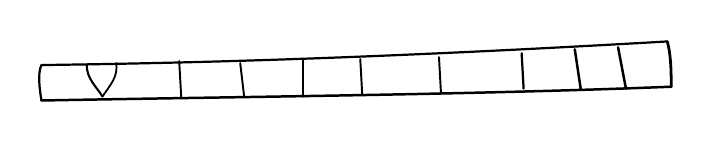
\begin{tikzpicture}[x=.025cm,y=-.025cm,line cap=round,line join=round]
\path[use as bounding box](10,5)rectangle(345,50);
\draw[line width=.8pt](17,24)..controls(88,23)and(179,21)..(335,12);
\draw[line width=.9pt](17,42)..controls(125,40)and(237,39)..(337,35);
\draw[line width=.8pt](17,24)..controls(15,28)and(16,36)..(17,42);
\draw[line width=1pt](335,12)..controls(337,19)and(337,29)..(337,35);
\draw[line width=.75pt](40,24)..controls(40,31)and(45,35)..(48,40);
\draw[line width=.65pt](55,23)..controls(56,30)and(52,34)..(48,40);
\draw[line width=.7pt](87,22)--(88,40);
\draw[line width=.7pt](118,23)--(120,40);
\draw[line width=.7pt](150,21)--(150,40);
\draw[line width=.7pt](179,21)--(180,39);
\draw[line width=.7pt](219,20)--(220,38);
\draw[line width=.8pt](261,18)--(262,36);
\draw[line width=.9pt](288,16)--(291,36);
\draw[line width=.9pt](310,15)--(314,36);
\end{tikzpicture}}}
Чем надо заниматься в дифф. ур-ях.
Для лин. опер. с кон. ядром и коядром ввод. индекс.
\begin{equation*}
k=\dim\ker T,\qquad
\ell=\dim\operatorname{coker}K,\qquad
\text{æ}=k-\ell.
\end{equation*}
\Unclear{GELFAND-P000035}{index-definition}{Буква после coker похожа на $K$. Петлевой знак индекса передан предварительным кандидатом æ; его точная буква не установлена.}
1) Если зам. на $\|T-T_1\|<\varepsilon$, то æ не мен.
2) Доб. \textcolor{orange!65!black}{вп. непр.}\ опер. не мен. индекса.
\Unclear{GELFAND-P000035}{compact-operator}{Написано Доб. вп. непр. опер.; слитные сокращения вп. непр. сохранены без раскрытия.}
æ позв. классиф. эллипт. ур-я на многообр.
(Атье и Зингер) Гомотопич. классифик.
Вишик счит., что индекс единств. гомотопич. инв.
\par\noindent\begin{minipage}{\linewidth}
Сист. с пост. коэфф. в шаре имеет [короткая запись зачёркнута]
как ещё один гомот. инв.
[Под строкой длинная зачёркнутая запись в скобках.]
\Unclear{GELFAND-P000035}{middle-cancellations}{После имеет короткая запись отменена; её нижняя петля видна. Ниже длинная запись в скобках зачёркнута двумя горизонтальными линиями; конец похож на инв. Текст не прочитан.}
\end{minipage}\par
Можно ли любую перев. в любую
(большого числа ур-й --- уст.).
Аналог. смысл имеет вопрос для раз. класса нелин. ур-й. Что такое æ?
Что такое ядро и коядро?
$\sim$ конечное ядро.
Квазилин. ур-е.
\begin{equation*}
Tu=v.
\end{equation*}
[Справа: $u$ --- многообр. Треб., чтобы оно было конечномерно.]
Главн. часть нелин. ур-я.
\underline{Коядро} $\sim$ [короткая волнистая линия].
[Справа: В кажд. точке линеариз. ур-е и везде одно и то же.]
\uwave{Задача}: исслед. индекс нелин. эллиптич. ур-я.
(Это вопрос интегральный.)
Квазилин.
\begin{equation*}
\sum A(\ldots u_0)\frac{\partial^2u}{\partial x^2}.
\end{equation*}
\Unclear{GELFAND-P000035}{nonlinear-formula}{Нижний знак при $u$ в аргументе $A$ похож на $0$ / $\omega$; слитные тёмные штрихи не дают точного выбора. Многоточие и отсутствие индексов суммы сохранены.}

\par\noindent\begin{minipage}{\linewidth}
\underline{\textcolor{orange!65!black}{16 го.}} Линник --- «\uwave{Как исп. ф. ан. в теории вероятностей}».
\Unclear{GELFAND-P000035}{linnik-date}{Мелкие знаки после 16 читаются предварительно как «го». Их начертание допускает чтение цифрами.}
\end{minipage}\par

\Needspace{5\baselineskip}
\par\noindent\begin{minipage}{\linewidth}
\SourcePage{GELFAND-P000036}{unlabelled}
\textcolor{orange!65!black}{И. И. / И. М.}\ Пятецкий-Шапиро.
\Unclear{GELFAND-P000036}{speaker-initials}{И. И. / И. М. Пятецкий-Шапиро. Второй инициал слит; точное чтение не установлено.}
\end{minipage}\par
(Илья Иосифович). \uwave{Раб. Линника.}
\begin{equation*}
x^2+y^2+z^2=m.
\end{equation*}
\par\noindent\begin{minipage}{\linewidth}
[Слева:] \textcolor{orange!65!black}{$\phi$}.
\Unclear{GELFAND-P000036}{left-sign}{На левом поле отдельный петлевой знак с правым вертикальным штрихом, похожий на $\phi$. Значение не подписано.}
\end{minipage}\par
При каком $m$ есть целочисл. решения?
Изв., что не всегда есть реш.
(При $m=8a+7$, то решений нет.) [Под $8a+7$: по mod 8.]
Как реш. расп. на пов. 3-х мерн. сферы.
Рад. $m^{1/2}$.
\SourceFigure{GELFAND-P000036}{sphere-projection}{Два неровных округлых контура, подписи $1$ и $\sqrt m$, расходящиеся линии, три жирные точки и утолщённый внутренний узел с маленькой стрелкой влево. Стык внутренних штрихов не вполне ясен.\par\smallskip\centering\color{black}\begin{tikzpicture}[x=.19mm,y=-.19mm,line width=.55pt]
\path[use as bounding box] (0,0) rectangle (325,260);
\draw (115,12) .. controls (162,4) and (204,38) .. (207,70) .. controls (228,125) and (183,187) .. (108,198) .. controls (35,206) and (0,137) .. (18,100) .. controls (19,55) and (65,12) .. (115,12);
\draw (113,78) .. controls (137,73) and (153,79) .. (153,94) .. controls (164,116) and (131,136) .. (107,130) .. controls (85,124) and (86,98) .. (90,90) .. controls (95,81) and (104,78) .. (113,78);
\draw (115,100) -- (145,87) -- (204,70);
\draw (115,100) .. controls (130,110) and (137,117) .. (152,117) -- (202,126);
\draw[line width=1pt] (112,98) -- (124,102) -- (131,99);
\draw (132,98) -- (123,102) -- (130,109);
\fill (115,100) circle (2);\fill (145,87) circle (2.8);\fill (204,70) circle (3);\fill (202,126) circle (3);
\node at (110,48) {$1$};\node at (255,137) {$\sqrt m$};
\end{tikzpicture}}
Выд. обл. на ед. сфере и посм., ск. точек в неё проецир.
\par\noindent\begin{minipage}{\linewidth}
\begin{equation*}
\frac{H_2(m)}{H(m)}\approx\operatorname{mes}\Omega.
\end{equation*}
\Unclear{GELFAND-P000036}{class-number-annotation}{Нижний знак в числителе похож на $2$; $\Omega$ остаётся альтернативой. Под $H(m)$: общ. число. Справа: \uwave{естеств. гипотеза}; ниже: но есть $m$, при к-рых мало. Последняя краткая запись не вполне ясна.}
\end{minipage}\par
\par\noindent\begin{minipage}{\linewidth}
Это справедливо при след. условии:
если прост. число $q$
\underline{$m$ \textcolor{orange!65!black}{пробег. / пробл.}\ числа:} $\xi^2+m=0\ (\operatorname{mod}q)$ разрешимо.
\Unclear{GELFAND-P000036}{q-condition}{Подчёркнуто: $m$ пробег. / пробл. числа. Средние и последние штрихи сокращения слитны; раскрытие не установлено.}
\end{minipage}\par
Для \textcolor{orange!65!black}{любой / небол.}\ такой послед. эта теор. справедлива.
\Unclear{GELFAND-P000036}{sequence-line}{Слитное слово после Для похоже на любой; затем такой послед. Прежнее чтение небол. остаётся альтернативой для тёмных начальных штрихов.}
С пом. $q$ на сфере устр. дин. система,
повед. к-рой подчин. вер. законам:
Фикс. $q$, рассм. [короткая запись зачёркнута] целую точку на сфере и все ортог. матрицы с эл. вида $a/q$.
\Unclear{GELFAND-P000036}{dynamics-cancellation}{Перед целую точку короткая запись зачёркнута несколькими густыми штрихами; текст не прочитан.}
($a$ --- целое.) Их кон. число, но много.
Целую точку они пер. в не целую.
Но среди них кон. число, перев. целую точку в целую.
Строим такой поток
($\forall$ точки свои $48$ ортог. матриц).
$e$ --- хар. ф-я.
\begin{equation*}
e(Tx)+e(T^2x).
\end{equation*}
[Стрелка вправо: \uwave{к площади}.]
Это марковская цепь.

\Needspace{5\baselineskip}
\par\noindent\begin{minipage}{\linewidth}
\SourcePage{GELFAND-P000037}{19}
\underline{Повзнер.} \underline{Наум Яковлевич.}
\uwave{План стат. физики.} \uwave{Инт. работы.}
\begin{equation*}
\begin{array}{ll}\text{Ruelle}&\text{2--3 раб.}\\\text{Yang Lee}&\text{1 раб.}\end{array}
\end{equation*}
\SourceFigure{GELFAND-P000037}{statistical-work-bracket}{Ломаная линия опускается ступенькой рядом со списком работ; её правая часть проходит под «Yang Lee».\par\smallskip\centering\begin{tikzpicture}[x=1mm,y=1mm,line width=.65pt]\draw (0,4)--(20,4)--(20,0)--(48,0);\end{tikzpicture}}
\end{minipage}\par
Это перевор. Всё, что изв. мат. по стат. физике.
Кац --- \uwave{модели}.
\underline{Задача.} (элем.)
\SourceFigure{GELFAND-P000037}{pair-potential}{Вертикаль с $u$, горизонталь с $0$ справа; кривая круто спускается ниже горизонтали, затем поднимается к ней справа. Правый участок утолщён. Слева: растёт. Точный стык утолщённых штрихов не вполне ясен.\par\smallskip\centering\color{black}\begin{tikzpicture}[x=.15mm,y=-.15mm,line width=.6pt]
\path[use as bounding box] (0,20) rectangle (465,250);
\draw (175,50) -- (181,210);
\draw (117,133) .. controls (175,142) and (310,129) .. (414,123);
\draw (191,50) .. controls (193,97) and (195,163) .. (203,183) .. controls (208,209) and (226,196) .. (250,168) .. controls (275,150) and (322,143) .. (370,135);
\draw[line width=1.7pt] (300,150) -- (333,142) -- (360,136);
\node at (159,41) {$u$};\node at (387,103) {$0$};\node at (70,75) {растёт};
\end{tikzpicture}}
\begin{equation*}
\min\sum_{i,j=1}^{N}u(x_i-x_j).
\end{equation*}
\SourceFigure{GELFAND-P000037}{configuration-bracket}{Линия под суммой поднимается ступенькой к записи справа.\par\smallskip\centering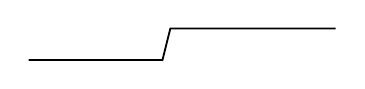
\begin{tikzpicture}[x=1mm,y=1mm,line width=.65pt]\draw (0,0)--(17,0)--(18,4)--(39,4);\end{tikzpicture}}
$x$ ходит в 2-мерн. пр-ве.\par
\underline{Набор $x$.}
Есть $C$, что min конфиг., что всё в сфере рад. $C$.
(Легко показ. $N^2$, а в случ. сферы $N^3$.)
[Под $N^2$ и «случ.» отдельные толстые линии.]

16/\underline{$\overline{\mathrm{XI}}$}
\underline{Лин. опер. в гильб. пр-ве имеет инв. подпр-во.}
Решена!!!
Bull. Amer. Math. Soc.
\par\noindent\begin{minipage}{\linewidth}
\uwave{\textcolor{orange!65!black}{Lui de Brange}} и \ldots
\Unclear{GELFAND-P000037}{de-brange-name}{Написано Lui de Brange и ...; окончание фамилии петлевое, возможен последний s. Год: 1964.}
\end{minipage}\par
1964.
Соед. с теор. Лившица.
\par\noindent\begin{minipage}{\linewidth}
[Слева ниже:] \textcolor{orange!65!black}{$\phi$ / $\psi$}.
\Unclear{GELFAND-P000037}{left-sign}{На левом поле отдельный знак с двумя верхними штрихами и правой нижней петлёй; графические кандидаты $\phi$ / $\psi$. Подписи нет.}
\end{minipage}\par
\underline{det} по Шуру.
Надо брать группу подст., а вместо всех --- \underline{предст.}
$\det$ + опр. матр. есть + опр. матрица.

\underline{Арнольд.}
Рассм. дин. сист. и соотв. квантовую сист.
\SourceFigure{GELFAND-P000037}{quantum-packet}{Почти круглый контур вокруг пересечения вертикали и горизонтальной стрелки вправо с подписью $x$. Внутри неровные вертикальные и волнистые штрихи; их пересечения местами слиты.\par\smallskip\centering\color{black}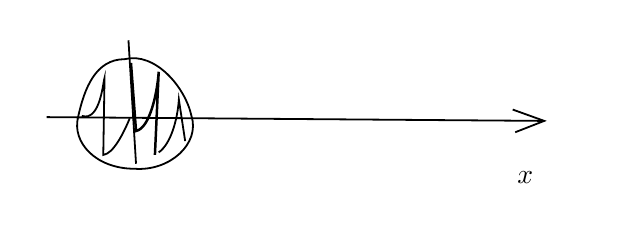
\begin{tikzpicture}[x=.16mm,y=-.16mm,line width=.65pt]
\path[use as bounding box] (0,30) rectangle (450,180);
\draw (15,101) -- (410,104);\draw (385,95) -- (410,104) -- (387,113);
\draw (80,40) -- (86,138);
\draw (77,55) .. controls (101,49) and (125,77) .. (130,100) .. controls (137,122) and (113,144) .. (85,142) .. controls (54,142) and (35,121) .. (40,101) .. controls (45,78) and (54,55) .. (77,55);
\draw (43,100) .. controls (58,105) and (60,71) .. (61,70) -- (60,131) .. controls (68,130) and (76,114) .. (81,102);
\draw[line width=.9pt] (82,58) -- (86,112) .. controls (97,110) and (103,81) .. (104,65) -- (101,131);
\draw (104,129) .. controls (114,122) and (119,102) .. (120,87) -- (125,120);
\node at (395,149) {$x$};
\end{tikzpicture}}
\begin{equation*}
\psi(x)e^{\frac{i}{h}S(x)}.
\end{equation*}
Квантовая частица.
\begin{equation*}
\psi\in\mathcal D(\mathbf R^n),\qquad S(x)=\int p\,dx.
\end{equation*}
$h$ --- пост. Планка.
Решение ищ. в таком же виде.
Получ. квазикл. асимптотика.
\SourceFigure{GELFAND-P000037}{bottom-trajectory}{Оси без подписей. Справа над горизонталью жирная точка; из неё дуга идёт вверх и вправо, затем вниз к правому наконечнику. Продолжение за границей кадра не показано.\par\smallskip\centering\color{black}\begin{tikzpicture}[x=.15mm,y=-.15mm,line width=.65pt]
\path[use as bounding box] (0,0) rectangle (455,195);
\draw (127,10) -- (118,160);\draw (29,140) .. controls (135,153) and (328,144) .. (431,157);
\fill (199,76) ellipse (7 and 10);
\draw (199,76) .. controls (229,43) and (281,35) .. (316,39) .. controls (356,39) and (375,62) .. (387,76);
\draw (378,54) -- (391,76) -- (365,79);
\end{tikzpicture}}

\Needspace{5\baselineskip}
\par\noindent\begin{minipage}{\linewidth}
\SourcePage{GELFAND-P000038}{unlabelled}
\begin{equation*}
\frac{\psi(\xi(x))e^{\frac{i}{h}(S(x)+\int p\,dx)}}{\sqrt{\dfrac{D(X)}{D(x)}}}.
\end{equation*}
\Unclear{GELFAND-P000038}{semiclassical-amplitude}{Аргумент $\psi$ переписан: $\xi(x)$ / $x$. Знак после $S(x)$ похож на $+$ / $t$. Под корнем верхняя буква аргумента похожа на $X$ / $x$; отдельного индекса не видно.}
\end{minipage}\par
[Справа: норм. множитель.]
Верна лишь при $h\longrightarrow0$, но при $D\ne0$.
(Через $t$ отобр. $D$ --- $\det$ новых т. по старым.)
Реш. вопр. прив. к топ. инвар. многообразия.
(В т. поворота.) \underline{Индекс.}
[Справа: При движ. получ. класс когомологий.]

\underline{Линник.}
\underline{Идеалы колец ф-й с точки зрения прилож. к статистике.}
A. Cartan --- о ид. колец голом. ф-й (47 и 50 г.).
Появл. аналит. пучки (снач. у \uwave{Ока}).
Прил. аппар. аналит. пучков.
Что такое статистика?
\begin{equation*}
(X,A,\mu)\overset{T}{\longrightarrow}(Y,B).
\end{equation*}
[Под первой скобкой: пр. с мерой. Под второй: пр-во с $\sigma$-сист.]
$T$ --- измер. отображение (ф-я наблюдений).
$X$ --- мы наблюдаем.
Мера на $Y$ прям. индуц. [короткая запись зачёркнута] из $X$.
\Unclear{GELFAND-P000038}{induced-measure-cancellation}{Между прям. индуц. и из $X$ короткая запись густо зачёркнута; точный текст не установлен.}
$X$ --- евкл. пр-во.
$A$ --- борелевы мн-ва.
\par\noindent\begin{minipage}{\linewidth}
$\mu$ --- мера.
(\textcolor{orange!65!black}{об. набор. мер, мажор. 1-й}).
\Unclear{GELFAND-P000038}{measure-parenthesis}{В скобках: об. набор. мер, мажор. / массы 1-й / 1-ой. Слитные штрихи перед 1-й ближе к мажор.; точное сокращение и окончание не установлены.}
\end{minipage}\par
\par\noindent\begin{minipage}{\linewidth}
Есть семейство мер $\left\{P(x,\theta)\right)$.
\EvidenceBlock{GELFAND-P000038}{family-delimiter}{После $P(x,\theta)$ стоит вторая круглая скобка.}{Запись в рукописи.}
\end{minipage}\par
[Под $P(x,\theta)$: зад. плотностью.]
Мы хотим получить свед. о параметре, наблюдая $X$.
\begin{equation*}
x_1,\ldots,x_n\in N(a,1).
\end{equation*}
[Под $N(a,1)$: гаусс. сем-во. Справа: 1 --- точность, $a$ --- параметр.]
\begin{equation*}
x_i=a+\Delta_i,\qquad\overline X\ \text{ср. арифм.}
\end{equation*}
$\Delta_i$ --- норм.

\Needspace{5\baselineskip}
\SourcePage{GELFAND-P000039}{20}
\underline{Стат.} --- нах. оценок.
Пров. гипотез $a=a_0$.
$\theta\in\Omega$.
($\Omega$ --- комп. в $\mathbf R^n$ обл.)
0-я гипотеза $H_0=\theta\in\omega$ (подпр-во).
\uwave{Пров. по пост. выборке с розыгрышем.}
Выб. тест --- ф-я наблюдений
\begin{equation*}
0\le\varphi(x_1,\ldots,x_n)\le1.
\end{equation*}
[Под формулой: вер. смысла.]
Наблюд. с пом. случ. ф-и и розыгрыш с пом. вер. $\varphi$, $1-\varphi$.
[Слева отмена и отдельный знак ниже.]
\Unclear{GELFAND-P000039}{test-cancellation}{Короткая запись густо зачёркнута. Под ней отдельно знак, похожий на $\pi$ / $\Pi$; значение не подписано.}
\par\noindent\begin{minipage}{\linewidth}
Прост. тест
\begin{equation*}
\varphi=\begin{cases}0\\1\end{cases}\qquad\begin{gathered}\text{отверг.}\\\text{или прин.}\end{gathered}
\end{equation*}
\EvidenceBlock{GELFAND-P000039}{simple-test-labels}{Две короткие записи расположены справа от $0$ и $1$. Прямых соединительных штрихов нет.}{Запись в рукописи.}
\end{minipage}\par
[Стрелка вниз к примеру:]
\begin{equation*}
|\overline x-a_0|>\varepsilon\qquad\text{отвергать или прин.}
\end{equation*}
\uwave{Качество теста оценив. так.}
\begin{equation*}
E(\varphi\mid H_0).
\end{equation*}
Мат. ожид. при гипотезе $H_0$ (парам. $\in\omega$).
[Справа: им. смысл лишь если 1 точка.]
$H_1$ --- альтернатива.
\par\noindent\begin{minipage}{\linewidth}
$\bigl(\overset{\theta}{H_1}\ \textcolor{orange!65!black}{\subset}\ \text{доп. }\omega\bigr)$.
\Unclear{GELFAND-P000039}{alternative-condition}{Над $H_1$ отдельно $\theta$. Следующий C-подобный знак может быть $\subset$; затем доп. $\omega$.}
\end{minipage}\par
\par\noindent\begin{minipage}{\linewidth}
\begin{equation*}
E(\varphi,H_a')\le\alpha,\qquad E(\varphi\mid H_1')=\max.
\end{equation*}
\Unclear{GELFAND-P000039}{null-expectation-subscript}{Слева нижний знак при $H$ похож на $a$ / $0$, верхний штрих на $\prime$ / $1$. Между $\varphi$ и $H$ запятая. Справа верхний штрих при $H_1$ виден отдельно.}
\end{minipage}\par
[Под левым ожиданием: простая гипотеза (зафикс. точка). Под правым: (желательно).]
Не слишком часто отвергали верную, но и часто отвергали
[короткая запись зачёркнута] неверную.
\Unclear{GELFAND-P000039}{lower-test-cancellation}{Перед неверную крохотный знак густо зачёркнут; текст под отменой не прочитан.}
\uwave{Тесты подобные.}
(В кажд. точке 0-й гипотезы вероятн. $\alpha$.)
\par\noindent\begin{minipage}{\linewidth}
\underline{Два примера.}
\SourceFigure{GELFAND-P000039}{gaussian-example-bracket}{Ступенчатая нижняя линия и высокий правый край окружают запись о гауссовой выборке.\par\smallskip\centering\resizebox{.98\linewidth}{!}{\begin{tikzpicture}[x=1mm,y=1mm,line width=.5pt]\node[anchor=north west,inner sep=0pt,text width=70mm] at (0,31) {$X$ распр. по Гауссу с ц. в неизв. точке $a_1$.\par $\sigma_1^2$ --- дисп.};\draw (0,0)--(47,0)--(47,5)--(75,5)--(75,33);\end{tikzpicture}}}
\end{minipage}\par
Пров. с пом. инв. тест.
\Unclear{GELFAND-P000039}{invariant-test-cancellation}{На продолжении: 0-я, ниже короткая отмена и гип. / ил. Слитные штрихи после отмены не дают точного чтения.}
\par\noindent\begin{minipage}{\linewidth}
$\theta$ --- \textcolor{orange!65!black}{мног.}\ $a_i$.
\Unclear{GELFAND-P000039}{theta-word}{$\theta$ --- мног. / мнот. $a_i$. Последний штрих сокращения похож на г / т; чтение не установлено.}
\end{minipage}\par
\underline{Вопр.} $a_1=a_2$?
\begin{equation*}
N(a_1,\sigma_1^2),\qquad x_1,x_2,\ldots,x_n,
\end{equation*}
\begin{equation*}
N(a_2,\sigma_2^2),\qquad y_1,\ldots,y_n.
\end{equation*}
[Справа: $\sigma_i^2$ --- парам. неизвестны.]
\begin{equation*}
H_0:\quad a_1=a_2,
\end{equation*}
\begin{equation*}
E(\varphi\mid H_0')=\alpha,\qquad E(\varphi\mid H_1)=\max.
\end{equation*}
$\varphi$ --- ?

\Needspace{5\baselineskip}
\SourcePage{GELFAND-P000040}{unlabelled}
$\varphi$ инв. или подобна, если $\forall\theta$ матем. ожидание $\varphi$ одно и то же.
($\forall\theta$ есть распр. вер.)
\par\noindent\begin{minipage}{\linewidth}
\begin{equation*}
E(\varphi\mid H_0)=\alpha,\qquad E(\varphi\mid H_1')=\max.
\end{equation*}
[Справа: \textcolor{orange!65!black}{[знак]}].
\Unclear{GELFAND-P000040}{right-hand-mark}{Справа от ожиданий виден отдельный густой знак. Его чтение не установлено.}
\end{minipage}\par
$H_1'$ --- одна точка в дополнении.
Байесова мера --- мера на пр-ве параметров.
(Зад. заранее --- априорное распред.)
[Слева стрелка вправо к строкам:]
Мера зав. от 4-ки точек $(a_1,a_2,\sigma_1,\sigma_2)$.
\underline{0-я гипотеза.}
\SourceFigure{GELFAND-P000040}{null-strip}{Под 0-я гипотеза неровная узкая полоса с наклонными штрихами; справа отдельно $a_1$ и запятая. Правые штрихи слиты с верхним краем.\par\smallskip\centering\color{black}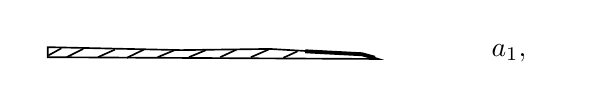
\begin{tikzpicture}[x=.075mm,y=-.075mm,line width=.6pt]
\path[use as bounding box] (0,30) rectangle (925,115);
\draw (34,63) -- (260,68) -- (410,66) -- (568,75) -- (594,83) -- (34,80) -- cycle;
\draw (35,77) -- (57,65) (66,80) -- (94,66) (119,80) -- (148,67) (168,81) -- (197,67) (220,80) -- (249,68) (273,80) -- (302,68) (326,80) -- (354,67) (378,80) -- (408,67) (433,81) -- (457,70);
\draw[line width=1.4pt] (470,70) -- (566,75) -- (588,81);
\node at (815,73) {$a_1,$};
\end{tikzpicture}}
\uwave{Байес. мера.}
\SourceFigure{GELFAND-P000040}{bayes-rectangle}{Рядом с Байес. мера пустой прямоугольник: верхняя сторона утолщена и выступает вправо, нижняя линия продолжается за обе вертикальные стороны. Внутри подписи нет.\par\smallskip\centering\color{black}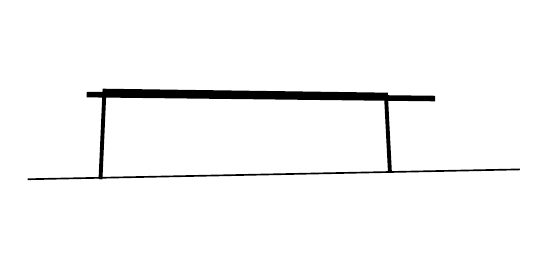
\begin{tikzpicture}[x=.25mm,y=-.25mm,line width=.6pt]
\path[use as bounding box] (0,0) rectangle (250,110);
\draw (0,77) -- (250,72);\draw[line width=1.4pt] (37,77) -- (39,32) -- (182,34) -- (184,73);
\draw[line width=2pt] (30,34) -- (207,36);
\end{tikzpicture}}
[Справа: Равном. распр., \textcolor{orange!65!black}{от.}\ $0$.]
\Unclear{GELFAND-P000040}{radon-measure-tail}{Краткая запись перед $0$ предварительно читается «от.».}
Надо уметь реш. $\forall$ байес. распр.-меры.
\underline{Рез.:} Распр. вер. в $X\times Y$ с зад. Гаусс. мерой (4-х парам.).
Надо найти $\varphi(x,y)$, чтобы
\par\noindent\begin{minipage}{\linewidth}
\begin{equation*}
E\bigl(\varphi(x_1,\ldots,x_{\textcolor{orange!65!black}{n}},y_1,\ldots,y_m)\bigr).
\end{equation*}
\Unclear{GELFAND-P000040}{sample-index}{Последний индекс при $x$ похож на $n$ или $m$; два штриха сливаются. При $y$ сохранено $m$.}
\Unclear{GELFAND-P000040}{gaussian-condition}{Справа: $\forall$ гаусс. допуст. мере ($=\alpha$ при $a_1=a_2$ и $\max$ проинтегр. на дополнении). Слово после $\max$ похоже на проинтегр.; параметр. остаётся прежним альтернативным чтением.}
\end{minipage}\par
\underline{Дост. статистика} --- сод. всю инф. о параметрах.

\underline{Не сделана зад.}
$\theta_1$, $\theta_2$ --- компл. перем.
$f(\theta_1,\theta_2)$ в шаре не известны \uwave{идеалы}
(Все прим. идеалы, отв. ид., равному 0.)
Глиссон --- шар и \uuline{центр} голом.
\par\noindent\begin{minipage}{\linewidth}
Дост. спец. идеалы ф-й, обр. в $0$ на \textcolor{orange!65!black}{$\theta$-х}\ кон. числе полиномов.
\Unclear{GELFAND-P000040}{terminal-ideals}{Первый знак после «на» предварительно прочитан как $\theta$; возможен $0$.}
\end{minipage}\par

\Needspace{5\baselineskip}
\SourcePage{GELFAND-P000041}{21}
Gleason — \underline{Горин.}

\par\noindent\begin{minipage}{\linewidth}
J. Math. Mech. v.~13. N~1 (1964).
\Unclear{GELFAND-P000041}{volume}{Поверх более ранних штрихов написано $13$. Нижнее число не установлено.}
\end{minipage}\par

Рассм. шар $z=(z_1,z_2)$,
\begin{equation*}
|z_1|^2+|z_2|^2\leq1
\end{equation*}
и ф-и, ан. внутри и непр. на гран., причём $f(0,0)=0$.
Сущ. ли $g_1,g_2$ того же типа, чтобы
\begin{equation*}
f=z_1g_1+z_2g_2
\end{equation*}
(max идеал; будет ли $z_1,z_2$ базисом?
Это можно сделать внутри, но неизв., можно ли на границе?
Для одной пер. тривиально.
Для бицилиндра делается (т.к. ряд Тейлора сх. на бицилиндре и можно взять \ldots).
Без гран. — тогда шар можно заменить любой областью голоморфности.

23/\underline{$\overline{\mathrm{XI}}$}. \underline{Арнольд.} «\uwave{О работе Маслова}».

Рассм. в частн. зад. Коши для ур-я Шредингера.
Конфиг. пр-во.
\par\noindent\begin{minipage}{\linewidth}
\begin{equation*}
\frac{i}{h}\frac{\partial\Psi}{\partial t}
=\Delta\Psi-\frac{U(x)}{h^2}\Psi
\end{equation*}
\Unclear{GELFAND-P000041}{schrodinger-factor}{Слева перед производной написано $i/h$; справа под $U(x)$ стоит $h^2$.}
\end{minipage}\par
$U(x)$ — потенц. энергия.
\SourceFigure{GELFAND-P000041}{potential-curve}{Над почти горизонтальной линией с правым наконечником $x$ стоит открытая сверху U-образная кривая; её дно не касается линии. Вертикальная ось не нарисована.\par\smallskip\centering\color{black}\begin{tikzpicture}[x=.12mm,y=-.12mm,line width=.55pt]\path[use as bounding box] (0,0) rectangle (540,230);
\draw (20,180) .. controls (130,180) and (320,167) .. (470,166);
\draw (447,156) -- (470,166) -- (448,178);
\node at (510,203) {$x$};
\draw (106,31) .. controls (119,115) and (139,143) .. (189,140) .. controls (255,144) and (273,113) .. (290,24);
\end{tikzpicture}}
\begin{equation*}
\left.\Psi\right|_{t=0}=\varphi(x)e^{\frac{i}{h}S(x)}
\end{equation*}
[Под $\varphi(x)$: фин.]
\SourceFigure{GELFAND-P000041}{initial-amplitude}{Над горизонтальной чертой небольшой округлый выступ с крутыми боками; справа сверху подпись $\varphi(x)$. Отдельные наконечники не различаются.\par\smallskip\centering\color{black}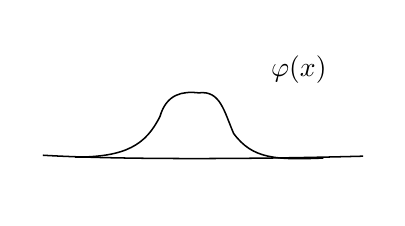
\begin{tikzpicture}[x=.12mm,y=-.12mm,line width=.55pt]\path[use as bounding box] (0,0) rectangle (370,180);
\draw (16,135) .. controls (100,140) and (246,139) .. (355,136);
\draw (50,137) .. controls (104,137) and (125,124) .. (140,94) .. controls (147,70) and (164,67) .. (181,69) .. controls (204,66) and (208,89) .. (218,112) .. controls (238,139) and (262,140) .. (313,138);
\node at (287,44) {$\varphi(x)$};
\end{tikzpicture}}
$S(x)$ может быть $S(x)=px$.
\SourceFigure{GELFAND-P000041}{wave-packet}{Между верхним и нижним округлыми контурами волнистые и почти вертикальные штрихи, пересечённые почти горизонтальной чертой. У краёв и в утолщениях отдельные соединения не разделяются уверенно.\par\smallskip\centering\color{black}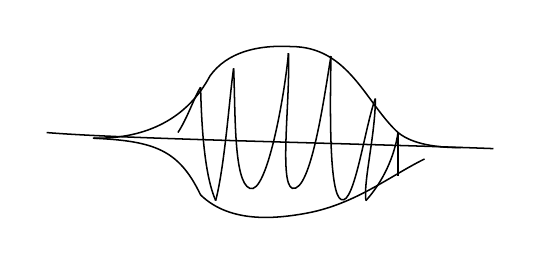
\begin{tikzpicture}[x=.12mm,y=-.12mm,line width=.55pt]\path[use as bounding box] (0,0) rectangle (505,220);
\draw (20,111) .. controls (105,118) and (335,122) .. (493,128);
\draw (69,117) .. controls (126,118) and (169,96) .. (193,51) .. controls (211,26) and (243,18) .. (279,20) .. controls (340,20) and (358,80) .. (392,111) .. controls (408,124) and (435,127) .. (459,127);
\draw (70,117) .. controls (134,120) and (160,129) .. (183,177) .. controls (215,208) and (265,202) .. (297,196) .. controls (348,186) and (385,156) .. (420,139);
\draw (159,111) .. controls (169,96) and (177,72) .. (183,63);
\draw (183,63) .. controls (184,104) and (187,156) .. (199,183);
\draw (199,183) .. controls (209,144) and (214,68) .. (218,43);
\draw (218,43) .. controls (220,92) and (218,163) .. (235,170) .. controls (253,178) and (272,72) .. (276,27);
\draw (276,27) .. controls (278,77) and (266,164) .. (280,170) .. controls (300,175) and (314,72) .. (321,30);
\draw (321,30) .. controls (320,90) and (319,177) .. (332,182) .. controls (346,188) and (357,104) .. (368,75);
\draw (368,75) .. controls (368,113) and (355,164) .. (358,183);
\draw (358,183) .. controls (376,163) and (388,137) .. (392,111);
\draw (392,111) -- (392,157);
\end{tikzpicture}}
\par\noindent\begin{minipage}{\linewidth}
Колеб. (быстрые), пропод.\ $\varphi$.
\Unclear{GELFAND-P000041}{caption-contraction}{После «Колеб. (быстрые)» написано «пропод.». Раскрытие сокращения не установлено. Затем $\varphi$.}
\end{minipage}\par

\Needspace{5\baselineskip}
\SourcePage{GELFAND-P000042}{unlabelled}
Асимпт. при $h\to0$ ищ. в виде
\begin{equation*}
\Psi=e^{\frac{i}{h}a(x,t)}.
\end{equation*}
$a$ — компл. ф-я.
Подставим и получ. послед. ас. ф-лы решения зад.
Первые 2 члена имеют вид
\par\noindent\begin{minipage}{\linewidth}
\begin{equation*}
\Psi(x,t)=
\frac{\varphi(X(x,t)}{\sqrt{\frac{\partial x(X,t)}{\partial X}}}
e^{\frac{i}{h}\left(S(X(x,t))+\int p\,dx\right)+O(h)}
\end{equation*}
\EvidenceBlock{GELFAND-P000042}{amplitude-delimiter}{В числителе после $t$ видна одна закрывающая скобка.}{Запись в рукописи.}
\Unclear{GELFAND-P000042}{remainder}{Запись $+O(h)$ стоит на поднятой строке после скобки фазы; отдельной нижней строки для неё нет.}
\Unclear{GELFAND-P000042}{amplitude-jacobian}{В числителе под корнем первый округлый знак похож на $D$ / $\partial$; в знаменателе виден $\partial X$. Верхний аргумент записан $(X,t)$.}
\end{minipage}\par
[От знаменателя: — из унит.; см. Титчмарш и Ландау.]
$\varphi$ — зад. нач. амплит.
$X$ при $t=0$ $=x$.
\par\noindent\begin{minipage}{\linewidth}
$\underset{(x,t)}{X}$ — [зачёркнуто: точка, из к-рой надо].
\Unclear{GELFAND-P000042}{cancelled-origin}{Под зачёркиванием читается точка, из к-рой надо / наше; последние буквы перекрыты чертой.}
\end{minipage}\par
Классич. нач. условие.
\par\noindent\begin{minipage}{\linewidth}
\begin{equation*}
p=\dot{x},\qquad \dot{x}=\frac{\partial S}{\partial x}
\end{equation*}
\Unclear{GELFAND-P000042}{classical-initial-signs}{У обоих знаков $x$ / $X$ видна точка сверху. После $\partial S$ нижний знак похож на $X$ / $x$; регистр не установлен уверенно. Отдельный нижний индекс у первого знака не виден.}
\end{minipage}\par
$S$ в нач. мом. задано.
\par\noindent\begin{minipage}{\linewidth}
$n$-мерн. \textcolor{orange!65!black}{пв. / пб.}
\Unclear{GELFAND-P000042}{dimensional-abbreviation}{После $n$-мерн. стоит короткое слитное сокращение, похожее на пв. / пб.; оно не раскрыто.}
\end{minipage}\par
\SourceFigure{GELFAND-P000042}{phase-figure}{Пересекающиеся почти горизонтальная и вертикальная линии, дуга над ними и две вертикальные черты от дуги. Под левой чертой $X$; $x$ стоит между чертами. Внутри вр. $t$. От левого пересечения наклонный штрих вправо вверх, с густым началом; направление стрелки не установлено.\par\smallskip\centering\color{black}\begin{tikzpicture}[x=.12mm,y=-.12mm,line width=.55pt]\path[use as bounding box] (0,0) rectangle (550,320);
\draw (28,223) .. controls (149,231) and (347,200) .. (528,193);
\draw (172,58) .. controls (167,119) and (164,210) .. (170,287);
\draw (206,184) .. controls (245,139) and (278,112) .. (302,107) .. controls (364,92) and (431,107) .. (488,141);
\draw (288,111) -- (390,76);
\draw (287,111) -- (294,211);
\draw (487,145) -- (487,155);\draw (487,162) -- (488,174);\draw (488,180) -- (489,192);
\draw[line width=1pt] (281,105) -- (297,115);\draw[line width=1pt] (288,102) -- (287,123);
\node at (285,271) {$X$};\node at (390,242) {$x$};\node at (370,145) {вр. $t$};
\end{tikzpicture}}
Ф-ла квазиклассич., справедл., когда якоб. $\neq0$.
\underline{Квазикл.} — когда справ. эта ф-ла.
\begin{equation*}
\ddot{x}=-\frac{\partial U}{\partial x}
\end{equation*}
классич. механика ($x$ — вектор).
В квант. мех. $\forall t$ есть волн. ф-я $\Psi$.
$|\Psi|^2$ — вер.
\par\noindent\begin{minipage}{\linewidth}
Ур-е движ. — Шрёд.
\begin{equation*}
\frac{i}{h}\frac{\partial\Psi}{\partial t}
=\Delta\Psi-\frac{U(x)}{h^2}\Psi
\end{equation*}
\Unclear{GELFAND-P000042}{schrodinger-factor}{В повторном уравнении слева $i/h$, справа $U(x)/h^2$; обе дроби видны отдельно.}
\end{minipage}\par
(если нет $i$, то ур-е теплопр.;
если нач. в точке, то потом расплывается).
Связ. с асимпт. соб. знач.
$\left.\Psi\right|_{t=0}$ задаётся. $\Psi(x)$
\SourceFigure{GELFAND-P000042}{terminal-line}{После $\Psi(x)$ длинная почти горизонтальная черта с утолщённым правым концом. Подписи над ней и уверенного наконечника нет.\par\smallskip\centering\color{black}\begin{tikzpicture}[x=.12mm,y=-.12mm,line width=.55pt]\path[use as bounding box] (0,0) rectangle (335,115);
\draw (0,71) .. controls (103,69) and (175,82) .. (280,75);
\draw[line width=.9pt] (276,73) -- (284,76);
\end{tikzpicture}}

\Needspace{5\baselineskip}
\SourcePage{GELFAND-P000043}{22}
$S(x)=px$ тогда ф-ла де Бройле.
\begin{equation*}
\frac{\partial S}{\partial x}=p
\end{equation*}
\par\noindent\begin{minipage}{\linewidth}
Обычн. приём нах. асимпт. — реш. ищ. в виде
\begin{equation*}
e^{\frac{i}{h}S_0(x^t)+S_1(x^t)+hS_2(x^t)+\cdots}
\end{equation*}
\Unclear{GELFAND-P000043}{exponent-variables}{Над $x$ во всех трёх аргументах поднятый знак с поперечной чертой, похожий на $t$; чтения $x^t$ / $\dot{x}$. Нижний знак у второго $S$ залит чернилами: $S_1$ / $S_0$.}
\end{minipage}\par
По времени [вписано сверху: дифф.] $\frac{1}{h^2}$ \ldots
Гл. член надо искать как $e^{\frac{i}{h}S_0(x)}$.
Если $S$ вещ., то осциллир., если компл., то есть уб.
Получ. ур-е 1-го пор. и 1-я ф-я вещ. и получ. осцилл.
Надо взять амплит., поэтому 2 чл.
Теперь надо подбр. нач. данные к этой асимпт.
\par\noindent\begin{minipage}{\linewidth}
$\Omega$ / $\delta$ нельзя, т.к. много постр. частот (сильно лок.).
\Unclear{GELFAND-P000043}{localized-datum}{$\Omega$ или $\delta$: петля с нижней горизонтальной чертой и длинным левым хвостом.}
\end{minipage}\par
\begin{equation*}
\varphi(x,t)e^{\frac{i}{h}S(x,t)}
\end{equation*}
если подст. туда, то для $S$ ур-е 1-го порядка
\begin{equation*}
\frac{\partial S}{\partial t}
=H\left(x,\frac{\partial S}{\partial x}\right),
\qquad H=U(x)+\frac{\dot{x}^2}{2}
\end{equation*}
к-рому соотв. обыкн. ур-е.
$\varphi$ — плотн. дин. сист. (как они движ. по кл. мех.).
Надо взять $x$ и для неё найти $X$, так что
наше ур-е через $t$ из $X$ придёт в $x$.
Точки несут с собой $\varphi$.
\SourceFigure{GELFAND-P000043}{trajectory}{Изгибающаяся кривая с $X$ под левым соединением и $x$ у правого конца. Через левое соединение проходит толстый наклонный штрих. Наконечник или направление не установлены.\par\smallskip\centering\color{black}\begin{tikzpicture}[x=.10mm,y=-.10mm,line width=.55pt]\path[use as bounding box] (0,0) rectangle (465,320);
\draw (30,275) .. controls (55,206) and (94,149) .. (130,110) .. controls (199,82) and (352,77) .. (433,129);
\draw[line width=.85pt] (130,110) -- (232,27);
\draw[line width=.85pt] (21,269) -- (37,280);
\draw[line width=.85pt] (429,124) -- (437,132);
\node at (180,145) {$X$};\node at (429,160) {$x$};
\end{tikzpicture}}
По $x$ дано $\dot{x}$ (дана дин. сист.).
При малых $t$ одн.
\begin{equation*}
\Psi=e^{iH}
\end{equation*}
унит.
$\mathcal{D}$ — якоб. доб. для унитарности.
$e$ — фаз. множ. с изм. амплит. крутится.
Раб. Маслова, когда $t$ произв., а не мало.
\par\noindent\begin{minipage}{\linewidth}
$t=0$ якоб. [запись зачёркнута] $=1$ (преобр. тожд.).
\Unclear{GELFAND-P000043}{cancelled-jacobian}{Густо зачёркнутое выражение после якоб. и перед $=1$; отдельные знаки не установлены.}
\end{minipage}\par
Волн. ф-я осциллятора. Маятник.
\SourceFigure{GELFAND-P000043}{oscillator}{Пересекаются параболическая дуга, колеблющийся контур, почти горизонтальная черта и центральный штрих. Видны $\varphi$, $0$, $x$; верхний небольшой знак похож на $\xi$, но его нижняя часть слита с кривой. Подписи: в кл. мех. волн. ф-я; $\exp$ убыв. Точные соединения густых штрихов и число колебаний не установлены.\par\smallskip\centering\color{black}\begin{tikzpicture}[x=.10mm,y=-.10mm,line width=.55pt]\path[use as bounding box] (0,0) rectangle (730,285);
\draw (45,139) .. controls (193,144) and (430,151) .. (586,155);
\draw (190,32) .. controls (189,106) and (208,144) .. (265,145) .. controls (323,148) and (374,108) .. (403,29);
\draw (68,135) .. controls (128,131) and (166,117) .. (185,76) .. controls (194,51) and (205,29) .. (215,30);
\draw (215,30) .. controls (229,29) and (226,77) .. (240,79) .. controls (253,83) and (262,29) .. (275,28) .. controls (287,26) and (280,77) .. (294,82) .. controls (303,87) and (312,54) .. (325,50) .. controls (344,43) and (351,82) .. (375,79) .. controls (389,79) and (398,61) .. (403,30);
\draw (190,67) .. controls (232,73) and (315,73) .. (384,72);
\draw (381,73) .. controls (402,105) and (426,124) .. (459,132) .. controls (508,149) and (549,150) .. (574,150);
\draw (280,29) .. controls (278,71) and (273,126) .. (265,162);
\draw (435,130) -- (432,193);
\node at (251,17) {$\varphi$};\node[text=orange!65!black] at (319,17) {$\xi\,?$};
\node at (280,183) {$0$};\node at (570,184) {$x$};
\node[anchor=west] at (431,54) {в кл. мех.};\node[anchor=west] at (460,89) {волн. ф-я};
\node at (525,226) {$\exp$ убыв.};
\end{tikzpicture}}

\Needspace{5\baselineskip}
\SourcePage{GELFAND-P000044}{unlabelled}
Если $t$ велико, то может случиться, что
кривая нач. данных ($n$-мерн. пв.) перемещается.
\SourceFigure{GELFAND-P000044}{folded-data}{Верхний левый рисунок: несколько загибающихся дуг пересечены наклонными штрихами, почти горизонтальной линией и густым почти вертикальным пучком. У верхнего левого конца и в пучке небольшие наконечники; отдельные соединения перекрыты.\par\smallskip\centering\color{black}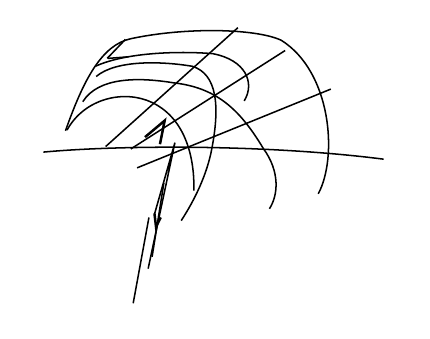
\begin{tikzpicture}[x=.10mm,y=-.10mm,line width=.55pt]\path[use as bounding box] (0,0) rectangle (475,360);
\draw (20,158) .. controls (117,149) and (304,148) .. (452,167);
\draw (48,131) .. controls (71,66) and (94,22) .. (131,14) .. controls (201,-1) and (290,1) .. (322,16) .. controls (386,56) and (394,165) .. (369,211);
\draw (70,94) .. controls (90,62) and (142,63) .. (185,70) .. controls (239,76) and (269,103) .. (299,153) .. controls (321,183) and (318,213) .. (307,230);
\draw (50,130) .. controls (72,90) and (122,78) .. (158,95) .. controls (206,118) and (212,177) .. (211,207);
\draw (87,62) .. controls (113,40) and (173,43) .. (209,49) .. controls (241,59) and (244,100) .. (234,153) .. controls (228,186) and (212,219) .. (195,245);
\draw (86,49) .. controls (128,30) and (199,30) .. (235,33) .. controls (277,41) and (289,70) .. (275,93);
\draw (101,39) -- (124,15);\draw (102,39) -- (128,37);
\draw (99,151) -- (267,0);
\draw (131,154) -- (327,29);
\draw (139,178) -- (385,78);
\draw (161,237) -- (187,146) -- (153,306);
\draw (173,197) -- (158,291);\draw (154,241) -- (134,350);
\draw[line width=.9pt] (149,139) -- (174,118) -- (168,148);
\draw[line width=.9pt] (169,241) -- (163,253) -- (161,236);
\end{tikzpicture}}
\par\noindent\begin{minipage}{\linewidth}
Если вертик. кас., то $\mathcal{D}=0$,
но потом 2 точки и ф-ла сохр. [(!) / (?)], но
надо доб. слаг. по точкам $\gamma_j$ / $n_j$ — целое.
\Unclear{GELFAND-P000044}{preserved-punctuation}{После сохр. маленький знак в скобках с отдельной нижней точкой: (!) / (?). Верхняя часть залита чернилами.}
\Unclear{GELFAND-P000044}{phase-integer}{$\gamma_j$ или $n_j$: у верхнего знака петля и два поднятых штриха; внизу $j$. Следующие записи имеют вид $n_j$.}
\end{minipage}\par
\par\noindent\begin{minipage}{\linewidth}
\begin{equation*}
\int p\,dx)+i\,\frac{\pi}{2}n_j
\end{equation*}
[Между $i$ и $\pi/2$ зачёркнут знак.]
\Unclear{GELFAND-P000044}{cancelled-phase-sign}{Между $i$ и $\pi/2$ густо зачёркнут знак; чтения $+$ / $-$ не установлены уверенно.}
\end{minipage}\par
\uwave{Рез. Маслова} — найдены \uuline{$n_j$}.
$n_j=\pm1$ из общих сообр.
Обойти около точки ветвл. в компл. плоскости,
этим можно сказ. $\oplus$ или $\ominus$.
Все рез. прим. и в \underline{оптике}.
\SourceFigure{GELFAND-P000044}{optical-rays}{Несколько наклонных лучей пересекаются с загибающейся огибающей. У верхнего касания толстая стрелка вправо вниз. На правой нижней ветви короткие пересекающиеся штрихи; их соединение с огибающей неуверенно.\par\smallskip\centering\color{black}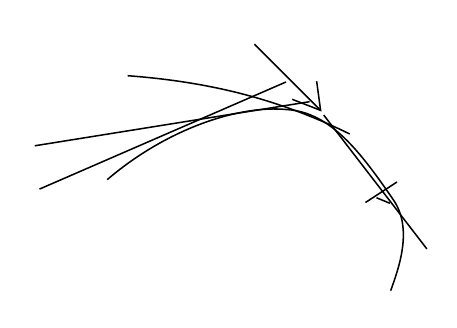
\begin{tikzpicture}[x=.10mm,y=-.10mm,line width=.55pt]\path[use as bounding box] (0,0) rectangle (510,345);
\draw (9,150) -- (358,94);
\draw (15,205) -- (328,69);
\draw (127,61) .. controls (233,69) and (319,91) .. (409,135);
\draw (101,193) .. controls (177,128) and (269,98) .. (329,104) .. controls (385,107) and (424,160) .. (464,218) .. controls (490,255) and (471,306) .. (461,334);
\draw (288,21) -- (372,105);\draw (336,91) -- (372,105) -- (367,68);
\draw (376,111) -- (507,281);
\draw (429,222) -- (469,196);\draw (443,216) -- (460,223);
\end{tikzpicture}}
Лучи огиб. кривую.
Будем следить за фазой по лучу.
При малых $\lambda$ — будет скачок фазы $\pi/2$ в точке касания.
\underline{Ответ} $n_j$ — индекс Морса.
\SourceFigure{GELFAND-P000044}{trajectory-figure}{Ось $p$ вверх, горизонтальная ось вправо. Семейство изогнутых и почти вертикальных штрихов; $x_1$, $x_2$, $X$. Подписи: кривая нач. данных; классич.; здесь вырожд.; через время $t$; через $t$; сопр. точки. Над центральной вертикалью густой небольшой знак; точное чтение и отдельные пересечения не установлены.\par\smallskip\centering\color{black}\begin{tikzpicture}[x=.065mm,y=-.065mm,line width=.55pt,every node/.style={font=\scriptsize,fill=white,inner sep=.4pt}]\path[use as bounding box] (0,0) rectangle (1080,545);
\draw (16,429) .. controls (277,427) and (545,431) .. (758,446);
\draw (716,430) -- (758,446) -- (714,463);
\draw (64,448) -- (57,153);\draw (45,174) -- (57,153) -- (70,174);
\node at (28,142) {$p$};
\draw[line width=.8pt] (184,412) .. controls (174,331) and (184,233) .. (213,186) .. controls (260,135) and (375,162) .. (441,165) .. controls (483,168) and (524,181) .. (551,210);
\draw[line width=.8pt] (177,356) .. controls (269,316) and (359,325) .. (429,349) .. controls (474,363) and (524,387) .. (569,437);
\draw (215,172) -- (295,118);
\draw (246,385) .. controls (256,304) and (288,210) .. (365,130);
\draw (352,389) .. controls (356,306) and (375,200) .. (415,145);
\draw (430,144) .. controls (418,229) and (420,345) .. (430,448);
\draw (453,167) .. controls (432,210) and (425,320) .. (430,395);
\draw (523,155) -- (522,389);
\draw (526,380) .. controls (497,320) and (486,242) .. (537,193) -- (585,155);
\draw (431,349) .. controls (461,317) and (478,273) .. (505,241);
\draw (378,450) .. controls (422,344) and (537,225) .. (683,179);
\draw (325,442) .. controls (362,382) and (402,357) .. (431,349);
\draw (513,409) -- (513,460);
\node at (130,363) {$x_1$};\node at (244,189) {$x_2$};\node at (518,503) {$X$};
\node[text=orange!65!black] at (435,143) {$?\!$};
\node[rotate=70] at (145,210) {нач. данных};
\node[rotate=68] at (270,55) {кривая};
\node[anchor=west] at (250,251) {классич.};
\node[anchor=west] at (686,158) {здесь вырожд.};
\node[anchor=west] at (568,260) {через время $t$};\node[anchor=west] at (607,350) {через $t$};
\node at (340,493) {сопр. точки};
\end{tikzpicture}}
Траект. — есть реш. вар. задачи по
принц. наим. действия.
\begin{gather*}
\delta u=0\\
\delta^2u
\end{gather*}
\par\noindent\begin{minipage}{\linewidth}
квадр. форма. У неё есть индекс [слово зачёркнуто]
(число отр. квадр.).
\Unclear{GELFAND-P000044}{cancelled-index}{Короткое слово слева от (число отр. квадр.) зачёркнуто густыми штрихами; чтение не установлено.}
\end{minipage}\par
\par\noindent\begin{minipage}{\linewidth}
Или [слово зачёркнуто] число сопряжённых точек.
\Unclear{GELFAND-P000044}{cancelled-conjugate}{Над число сопряжённых точек слово закрыто несколькими горизонтальными штрихами; чтение не установлено.}
\end{minipage}\par
1-я часть раб. \underline{Лере} посв. близким вопр.
\par\noindent\begin{minipage}{\linewidth}
След. раз Повзнер Yang Lee и \textcolor{orange!65!black}{Брушлин}.
\Unclear{GELFAND-P000044}{next-speakers}{В строке читается «Yang Lee». Над «Lee» короткая приписка, похожая на «группам». Последняя фамилия предварительно читается «Брушлин».}
\end{minipage}\par

\Needspace{5\baselineskip}
\SourcePage{GELFAND-P000045}{23}
\underline{Березин.}
\begin{equation*}
H=\frac{p^2}{2}+V(x)
\end{equation*}
(напр. $V$ — растёт).
Пусть пов. $p^2+V(x)=\mathrm{const}$ все ограничены.
\par\noindent\begin{minipage}{\linewidth}
Тогда асимпт. собств. [сокращение зачёркнуто] значений:
\Unclear{GELFAND-P000045}{cancelled-eigenfunction}{Перед значений зачёркнутое сокращение похоже на ф-й / ф-и; верхние буквы пересечены горизонтальными штрихами.}
\end{minipage}\par
\par\noindent\begin{minipage}{\linewidth}
объём обл., где $H\leq n\pi h$ — асимптотика
[слово зачёркнуто] соб. чисел.
\Unclear{GELFAND-P000045}{cancelled-asymptotic}{Между асимптотика и соб. чисел короткое слово закрыто густыми чернилами; чтение не установлено.}
\end{minipage}\par
\par\medskip{\centering\rule{12mm}{.45pt}\enspace$\cdot$\enspace\rule{15mm}{.45pt}\par}\medskip
\underline{Гельфанд И.}
\begin{equation*}
-y''+p(x)y=\lambda y
\end{equation*}
\SourceFigure{GELFAND-P000045}{wavefunction-diagram}{Горизонтальный отрезок с короткими конечными штрихами и подписями $0$, $\pi$. Одна дуга над отрезком; другая кривая сначала над ним, затем пересекает его и уходит вниз. Возле правого конца густое соединение; расположенное рядом подчёркивание на концах 0 перечёркнуто.\par\smallskip\centering\color{black}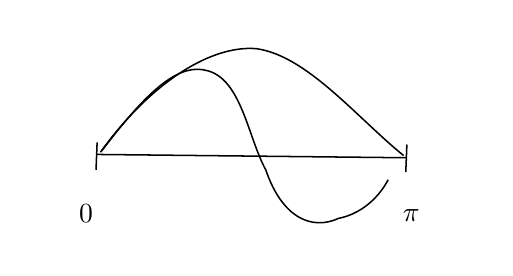
\begin{tikzpicture}[x=.14mm,y=-.14mm,line width=.55pt]
\path[use as bounding box] (0,0) rectangle (415,200);
\draw (63,115) -- (344,118);
\draw (63,104) -- (62,129);\draw (344,106) -- (343,131);
\draw (66,113) .. controls (113,48) and (167,16) .. (207,19) .. controls (253,25) and (298,81) .. (341,116);
\draw (67,112) .. controls (111,54) and (138,32) .. (163,39) .. controls (194,47) and (200,100) .. (216,129) .. controls (231,173) and (258,184) .. (282,173) .. controls (302,169) and (318,155) .. (327,138);
\node at (53,169) {$0$};\node at (348,170) {$\pi$};
\end{tikzpicture}}
\underline{На концах 0} [подчёркивание перечёркнуто].
\par\noindent\begin{minipage}{\linewidth}
$p=0$, собств. ф-и, $\lambda=-n^2$.
\Unclear{GELFAND-P000045}{lambda-sign}{В записи $\lambda=-n^2$ отдельная горизонтальная черта между знаком равенства и $n$ видна; минус сохранён.}
\end{minipage}\par
Утв. 1-я соб. ф-я не им. 0-й (инд. Морса 1).
2-я —//— им. один 0.
Это верно $\forall$ ур-ю.
Нули перемежаются.
Более точная теор. Если $y_0,\ldots,y_n$ соб. ф-я,
то
\begin{equation*}
\sum_{i=1}^{n}a_i y_i(x)
\end{equation*}
будет иметь $\leq n$ нулей!!
(похоже на многочлены).
\par\noindent\begin{minipage}{\linewidth}
[Зачёркнут определитель:]
\begin{equation*}
\det\begin{vmatrix}
y_0(x)&y_1&\cdots\\
y_0'(x)&y_1'&\\
\vdots&\vdots&\\
y_0^{(n)}(x)&y'(x)&
\end{vmatrix}
\end{equation*}
\Unclear{GELFAND-P000045}{cancelled-determinant}{В зачёркнутом определителе нижний второй элемент похож на $y\prime(x)$ / $y_1^{(n)}(x)$; индекс и порядок производной не установлены.}
\end{minipage}\par
\par\noindent\begin{minipage}{\linewidth}
Это экв. условию
\begin{equation*}
\begin{vmatrix}
y_0(x_0)&y_1(x_1)&\cdots\\
y_0'(x_0)&y_1'(x_1)&\cdots\\
\vdots&\vdots&\\
y_0^{(n)}(x_0)&y_1'(x_1)&
\end{vmatrix}\neq0
\end{equation*}
\Unclear{GELFAND-P000045}{mixed-determinant}{Во втором элементе второй строки переписан верхний знак у $y_1\prime(x_1)$. В нижнем втором элементе виден один поднятый штрих: $y_1\prime(x_1)$; возможный порядок $(n)$ не установлен.}
\end{minipage}\par
\par\noindent\begin{minipage}{\linewidth}
Или
[Над следующим определителем:] это 1-я соб. ф-я ур-я 2-го пор., к-рая $\neq0$.
\begin{equation*}
\begin{vmatrix}
y_0(x_0)&y_1(x_0)&\cdots\\
y_0(x_1)&y_1(x_1)&\cdots\\
\vdots&\vdots&\\
y_0(x_n)&y_0(x_n)&
\end{vmatrix}\neq0
\end{equation*}
\Unclear{GELFAND-P000045}{value-determinant}{Во втором элементе нижней строки индекс округлый, как у $y_0$ в первом столбце. Точка сверху совпадает с вертикальным многоточием; отдельный штрих производной не установлен.}
\end{minipage}\par
Отсюда лин. комб. $\leq n$ нулей, если $x_0<x_1<\cdots<x_n$.
\par\noindent\begin{minipage}{\linewidth}
Петров. чтобы
\begin{equation*}
\begin{aligned}
\frac{\partial^2u}{\partial x_1^2}
-\frac{\partial^2u}{\partial x_2}-\cdots
+\left(p(x_1)+p(x_2)\ldots+p(x_n)\right)u&={}\\
&=\lambda u
\end{aligned}
\end{equation*}
\Unclear{GELFAND-P000045}{petrov-equation}{В первом знаменателе $x_1^2$, во втором виден $x_2$ без квадрата. Справа на краю $u=$; ниже ещё один знак равенства перед $\lambda u$. Оба знака сохранены.}
\end{minipage}\par
Соб. ф-и перем. разделяются.
Соб. ф-и $u_1(x_1)u_2(x_2)\ldots u_n(x_n)$.
1-я соб. ф-я $\neq0$.

\Needspace{5\baselineskip}
\par\noindent\begin{minipage}{\linewidth}
\SourcePage{GELFAND-P000046}{unlabelled}
\par\medskip{\centering\rule{12mm}{.45pt}\enspace$\cdot$\enspace\rule{15mm}{.45pt}\par}\medskip
\uwave{Намечено}. [Номер и инициалы неясны] Бернштейн и С. Гильфанд.
\Unclear{GELFAND-P000046}{planned-speakers}{Начало первой строки: длинный петлеобразный знак, затем И / Н перед Бернштейн. Чтения: $1^\circ$ И. Бернштейн и С. Гильфанд / Ф. Н. Бернштейн и С. Гильфанд / $1^\circ$ И. Бернштейн и С. Гельфанд. Полные имена не установлены.}
\end{minipage}\par
[Справа отдельно:] \uwave{Дайсон}.
$2^\circ$. Новиков, о раб. \uwave{Адамса}.
$3^\circ$. Дынкин.
$4^\circ$. Винберг.
$5^\circ$. Пятецкий-Шапиро.
\par\noindent\begin{minipage}{\linewidth}
[Зачёркнуто.]
\Unclear{GELFAND-P000046}{cancelled-heading}{Короткий зачёркнутый и дважды подчёркнутый заголовок перед Пят.-Шапиро похож на Пят.; прежние штрихи густо перекрыты.}
\end{minipage}\par
\underline{Пят.-Шапиро}.
Зад. Клейна и Серра.
Рассм. гр. целочисл. матриц $n$-го пор. $\Gamma(n)$ с $\det=1$.
[Зачёркнуто: Как]
опис. все подгр. $\Gamma'$ конечного индекса?
\underline{Прим.}
\par\noindent\begin{minipage}{\linewidth}
\begin{equation*}
\Gamma(n,N),\qquad A\equiv E\pmod N
\end{equation*}
\Unclear{GELFAND-P000046}{congruence-index}{Под $\Gamma(n,N)$ мелкая подпись, похожая на $\lambda ij$ / $i,j$; под $A\equiv E$ — вероятно «не гр.», возможно «на гр.» Буквы и принадлежность маленькой подписи к формуле не установлены.}
\end{minipage}\par
(на диаг. сравн. с $1$, а вне диаг. делится на $N$).

\Needspace{5\baselineskip}
\SourcePage{GELFAND-P000047}{35}
Все ли это подгруппы?
Всегда ли $\Gamma'$ содержит $\Gamma(n,N)$
(конгруенц.-подгруппу).
При $n=2$ это не так (Клейн).
$n\geq3$ это так (Серр).
\underline{Связь с группами Ли.}
Рассм. матрицы
\SourceFigure{GELFAND-P000047}{elementary-stencil}{Схема матрицы.\par\smallskip
\centering\color{black}
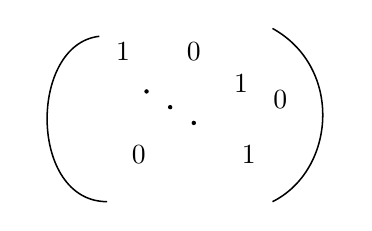
\begin{tikzpicture}[x=1mm,y=-1mm,line width=.55pt]
\draw (9,2) .. controls (0,3) and (0,23) .. (10,23);
\draw (31,1) .. controls (40,6) and (39,19) .. (31,23);
\node at (12,4) {$1$};\node at (21,4) {$0$};
\node at (27,8) {$1$};\node at (32,10) {$0$};
\fill (15,9) circle (.28);\fill (18,11) circle (.28);\fill (21,13) circle (.28);
\node at (14,17) {$0$};\node at (28,17) {$1$};
\end{tikzpicture}}
\par\noindent\begin{minipage}{\linewidth}
[Зачёркнут символ.]
\Unclear{GELFAND-P000047}{cancelled-elementary}{Перед обозначением элементарной матрицы зачёркнут и переписан знак, похожий на $E$; нижние штрихи не установлены.}
\end{minipage}\par
\par\noindent\begin{minipage}{\linewidth}
$E_{ke}=(\mathrm{ед.}+E_{ke})$.
\Unclear{GELFAND-P000047}{elementary-matrix}{С обеих сторон равенства один и тот же $E$-образный знак; второй нижний индекс похож на $e$ / $\ell$. Чтения $E_{ke}=(\text{ед.}+E_{ke})$ / $e_{k\ell}=(\text{ед.}+E_{k\ell})$. В схеме сохранены видимые единицы, нули и точки; незаписанные элементы не дополнены.}
\end{minipage}\par
\underline{Гр. $\Gamma(n)$ ими порождается}.
Возьмём эти матр. и сопр. и возв. в степ. $N$:
$E_{ke}^{N}$, $\Gamma^{N}$.
При $n=2$ она беск. индекса;
$n\geq3$ кон. индекса.
$\Gamma/\Gamma^{N}$.
\fbox{$n=2$}
\par\noindent\begin{minipage}{\linewidth}
$N=2,3,4,5$ конечна, 6 \textcolor{orange!65!black}{коммут. / коннут.}
\Unclear{GELFAND-P000047}{surface-abbreviation}{После 6 сокращение коммут. / коннут. Начальная буква имеет раздельные вертикальный и угловатый штрихи. Ниже $p=p(N)$; буква похожа на $p$. Сокращение не раскрыто.}
\end{minipage}\par
$\Gamma/\Gamma^{N}=$ фунд. гр. поверхности,
$p=p(N)$, простая формула.
Серр, Лазар, Басс (1964).
\par\noindent\begin{minipage}{\linewidth}
Рассм. $a\equiv b\ (N)$, тогда при $n\geq3$ / $N\geq3$
в $\Gamma/\Gamma^{N}$ есть преобр. $a\to b$ (элем. преобраз.).
\Unclear{GELFAND-P000047}{rank-overwrite}{После тогда при знак перед $\geq3$ густо переписан: $n\geq3$ / $N\geq3$. Видны вертикальные штрихи, похожие на прописное $N$.}
\end{minipage}\par
Потом когом. техника.

\underline{Гельфанд.}
Завтра на конф. по элем. частицам будет расск.
\par\noindent\begin{minipage}{\linewidth}
[Зачёркнуто.]
\Unclear{GELFAND-P000047}{cancelled-particles}{Перед обведённым $SU(3)$ густо зачёркнуто обозначение группы. Чтения $SU(3)$ / $SU(2)$; цифра под чернилами не установлена.}
\end{minipage}\par
\fbox{$SU(3)$}.
Изв.-част. объед. в группы, преобр. друг в друга (мультиплеты).
Другая предст. $SU(3)$.
Идея $SU(2)\underset{\text{почти}}{\approx}SO(3)$.
[Над строкой: фн. лин. комб.]
Объед. с помощью 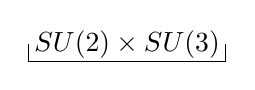
\begin{tikzpicture}[baseline=(product.base)]\node[inner xsep=2pt,inner ysep=1pt] (product) {$SU(2)\times SU(3)$};\draw (product.west) -- (product.south west) -- (product.south east) -- (product.east);\end{tikzpicture}.
Гипотеза изв. и по $SU(6)$.
\underline{Замеч.} — в самом деле Лоренц. группа (с пар. перемещ.)
(группа Пуанкаре).
[Зачёркнуто: $SU(2)$] $\longrightarrow$ гр. Пуанкаре.
Раб. \underline{Тодорова}.
\uwave{Кадышевский}, \uwave{Мурадян}, \uwave{Тавхелидзе}.
Вместо $SU(6)$ — 108 парам. группу.

\Needspace{5\baselineskip}
\SourcePage{GELFAND-P000048}{unlabelled}
Salam предл. 144-пар. группу.
Fulton, Wess.
Гр. 2-х ступ. с комм. норм. делителем.
\par\noindent\begin{minipage}{\linewidth}
$SU(3)\otimes SU(2)$ в как. смысле.
\Unclear{GELFAND-P000048}{in-some-sense}{Сокращение перед смысле похоже на как. или нек.}
\end{minipage}\par
Лор. преобр. — компл. матр.
\begin{equation*}
\begin{pmatrix}\alpha&\beta\\\gamma&\delta\end{pmatrix},
\qquad \det=1
\end{equation*}
(спинорное предст. гр. Лоренца).
Гр. \uwave{Пуанкаре}\enspace\rule[-.28em]{.6pt}{1.4em}
\begin{equation*}
A=\begin{pmatrix}\alpha&\beta\\\gamma&\delta\end{pmatrix}
\end{equation*}
\uwave{Вектор} — эрм. формы 2-го пор.
\begin{equation*}
H=\begin{pmatrix}a&b\\\bar b&c\end{pmatrix}
\end{equation*}
век. в 4-х мерн. пр-ве; $a,c$ — вещ., $b$ — компл.
\begin{equation*}
H\to AHA^*
\end{equation*}
Лор. $\det$ сохр.
Гр. Пуанкаре
\begin{equation*}
\begin{pmatrix}A&H\\0&A^{*-1}\end{pmatrix}
\end{equation*}
\par\noindent\begin{minipage}{\linewidth}
Это группа при $H\geq0$ / $H=0$ вращ. ($H$ склад.).
$H=1$ — пар. перем.
\Unclear{GELFAND-P000048}{h-zero}{Условие на $H$: перед $0$ верхний угловатый и нижний горизонтальный штрих; чтения $H\geq0$ / $H=0$.}
\end{minipage}\par
\par\noindent\begin{minipage}{\linewidth}
[Зачёркнуто.]
\Unclear{GELFAND-P000048}{cancelled-group}{Перед Матр. 4-го порядка зачёркнута фраза, начинающаяся гр.; следующее слово похоже на Вращ. / Лоренца.}
\end{minipage}\par
Матр. 4-го порядка.
\begin{equation*}
\underline{\begin{pmatrix}A&H\\0&A^{*-1}\end{pmatrix}}\otimes SU(3)
\end{equation*}
\par\noindent\begin{minipage}{\linewidth}
получ. полупрост. гр. с \textcolor{orange!65!black}{разреш.} (108-парам.).
\Unclear{GELFAND-P000048}{group-abbreviation}{Сокращение после с похоже на разреш.; окончание слито.}
\end{minipage}\par
Можно опис., что \underline{нужно}, \underline{чтобы} реш. теор. элем. частиц).

15/II\par\underline{Каждан}.
Рез. Палам. в чисто алг. терминах.
\par\noindent\begin{minipage}{\linewidth}
Пусть $A$ — [зачёркнуто, сверху вписано: область]
целостности (кольцо без дел. нуля), $I$ — прим. идеал.
\Unclear{GELFAND-P000048}{domain-cancellation}{Область вписано над зачёркнутым словом; кандидат кольцо. Густые штрихи не позволяют установить всё слово. Следующее целостности (кольцо без дел. нуля) читается.}
\end{minipage}\par
\par\noindent\begin{minipage}{\linewidth}
\begin{equation*}
I\supset J
\end{equation*}
[Под $J$:] простой.
И пусть $J\supset I^2$ [зачёркнуто: $\neq$] $0$.
\Unclear{GELFAND-P000048}{ideal-powers}{$I$ введён как прим. идеал; под $J$ в $I\supset J$ написано простой. Затем $J\supset I^2$, перед $0$ зачёркнут знак, похожий на $\neq$. Буквы и зачёркивание сохранены.}
\end{minipage}\par
Каждый такой идеал зад. дифф. \underline{опер. \underline{1-го пор.}}

\Needspace{5\baselineskip}
\par\noindent\begin{minipage}{\linewidth}
\SourcePage{GELFAND-P000049}{36}
Дифф. опер. — $A$ / $K$ / $k$-лин. опер.
\Unclear{GELFAND-P000049}{linear-glyph}{Густо переписанный знак перед -лин. похож на $A$ с выступающим верхним штрихом. Возможны $K$ и $k$.}
\end{minipage}\par
\par\noindent\begin{minipage}{\linewidth}
\begin{equation*}
D(a\cdot b)=aD(b)+D(a)b
\end{equation*}
\Unclear{GELFAND-P000049}{product-comma}{Под точкой умножения в аргументе $D$ виден отдельный знак, похожий на запятую.}
\end{minipage}\par
Идеал — 0 нек-рого наб. дифф. опер.
Пусть $A/J^2$ (1-го пор. из-за $J^2$).
Оператор не в кольцо, а в кольцо $A/J$.
Дифф. всюду, а отв. на подмн.
$aD(b)$ — умн. на $a$.
На $J$ опер. $A$-линейный [снизу: дифф.].
Наоборот, каждый $A$-лин. опер. на $J$
\par\noindent\begin{minipage}{\linewidth}
[Зачёркнутый знак перед $J$]:
\Unclear{GELFAND-P000049}{cancelled-map-strokes}{Слева от $J$ три густых почти вертикальных зачёркнутых штриха с петлёй; за ними двоеточие. Отдельная буква под ними не установлена.}
\begin{equation*}
J\overset{f}{\longrightarrow}A/J
\end{equation*}
\end{minipage}\par
Тогда его можно домн. на элем. $b$, снова лин.
[Сверху: $bf$.]
$\exists b$, что $bf$ продолжается до дифф. всего кольца.
Отсюда всё следует.
\par\noindent\begin{minipage}{\linewidth}
Будем рассм. $J(2)$ / $J(\xi)$ / $J(\ell)$ над полем частных.
\Unclear{GELFAND-P000049}{field-notation}{После $J$ знак в скобках похож на $2$ / $\xi$ / $\ell$, затем над полем частных. Чтения $J(2)$ / $J(\xi)$ / $J(\ell)$.}
\end{minipage}\par
Сущ. функционалы, вид. $J$ леж. в кольце частных.
\par\noindent\begin{minipage}{\linewidth}
Домн. на $b$ (т.к. нет дел. 0, то [зачёркнут короткий знак] кольцо ч.).
\Unclear{GELFAND-P000049}{cancelled-field-symbol}{Между то и кольцо ч. короткий густо зачёркнутый знак; чтение не установлено.}
\end{minipage}\par
Если $A/J$ поле, тогда $\forall$ ф-л прод. до диффер.
(Надо взять локализацию $A/J$).
Сущ. отобр. поля
\begin{equation*}
A/J\longrightarrow A
\end{equation*}
[Под стрелкой: гом.]
чтобы обр. гом. был тождеств.
\begin{equation*}
A/J\longrightarrow A\longrightarrow A/J
\end{equation*}
\par\noindent\begin{minipage}{\linewidth}
[Зачёркнуто.]
\Unclear{GELFAND-P000049}{cancelled-word}{Зачёркнутый заголовок перед Пока произв. похож на Док-во.; чтение остаётся неуверенным под перечёркиванием.}
\end{minipage}\par
Пока произв.
$A/J\subset A$, $J\subset A$.
Любой эл. расклад. в $\Sigma$ ($\Sigma$ как лин. пр-во).

\Needspace{5\baselineskip}
\SourcePage{GELFAND-P000050}{unlabelled}
На $J$ он уже задан.
Лин. отобр. $J\to A/J$ прод.
\par
На всём $0$.
\par
Трансценд. эл. куда угодно.
\par\noindent\begin{minipage}{\linewidth}
\begin{gather*}
y\to\hat y,\qquad x^2=y\\
\hat x'^{\,2}-\hat y=i_1;\qquad
\hat x=\hat x'+i_2;\\
\hat x^2=\hat x'^{\,2}+2\hat x'i_2
=\hat y+2\hat xi_2+i_1
\end{gather*}
\Unclear{GELFAND-P000050}{square-expansion}{В разложении нет $i_2^2$. В первом равенстве множитель $\hat x\prime$, во втором $\hat x$ без штриха. Обе записи сохранены.}
\end{minipage}\par
Отсюда $i_2$ находится (т.к. $A/J$ поле).
Вместо $I$ писалось $J$ и наоборот.
\par\medskip{\centering\rule{12mm}{.45pt}\enspace$\cdot$\enspace\rule{15mm}{.45pt}\par}\medskip
Общ. вид дифф. опер. в кольце мног.
\begin{equation*}
\sum P_i(x_1,\ldots,x_n)\frac{\partial}{\partial x_i}
\end{equation*}
$P_i$ — многочлены.
\uwave{Алгебр. теория дифф. ур-й} \uwave{над произв. полем}.
Дьёдонне, Гротендик: перешли в алг. зад. к произв. полю.
\par\noindent\begin{minipage}{\linewidth}
\underline{Обыкн. ур-е.}
\begin{gather*}
\frac{dx}{dt}=P(x,y)\\
\frac{dy}{dt}=Q(x,y)
\end{gather*}
\Unclear{GELFAND-P000050}{overwritten-numerator}{В числителе первого уравнения буква густо переписана; видимый кандидат $dx$, прежняя буква не установлена.}
\end{minipage}\par
$t$ замен. лок. кольцом $\forall$ точке ($t$ лок. параметр).
\begin{gather*}
x=\sum a_k t^k\\
y=\sum b_k t^k
\end{gather*}
\par\noindent\begin{minipage}{\linewidth}
Дифф. \underline{ур-я над $P^2$.}
\Unclear{GELFAND-P000050}{differential-field}{Подчёркнутая буква, похожая на $P$, с поднятой $2$: $P^2$ / $p^2$. Двойной штрих не виден.}
\end{minipage}\par
\begin{equation*}
D(x(t))=f(x(t))
\end{equation*}
$D$ — дифф. оператор в кольце элем. $x$.
Окольцованное пр-во. Точки $(x,y)$ и \uuline{слои}.
$\forall$ точке кольцо.
Слой над каждой точкой — степ. ряд от $t$
($\forall$ точке степ. ряд от $t$).

\Needspace{5\baselineskip}
\SourcePage{GELFAND-P000051}{37}
\begin{equation*}
Da=b.
\end{equation*}
\Unclear{GELFAND-P000051}{upper-equation-letter}{В левой записи $a$ / $\alpha$; отдельного определения на этом кадре нет.}
Нач. усл. --- знач. в макс. идеале.
Потом локализовать.
$D$ перен. на любую локализацию.
Реш. должно быть идеалом. (?)
Всё кольцо не надо зад. Оно изв. локально.
$x$ и $y$ не надо задавать.

\underline{Паламодов.}
\begin{equation*}
\mathcal P\quad\text{--- кольцо мн.}\qquad P(z_1,\ldots,z_n)
\end{equation*}
[Перед $P$: знак зачёркнут.]
\Unclear{GELFAND-P000051}{polynomial-cancellation}{густо зачёркнут короткий символ}
$\mathcal H$ --- пр-во всех ф-й в обл. голом. (напр. шар)
\begin{equation*}
\mathcal J\subset\mathcal P
\end{equation*}
Прим. идеал с базисом $P_1,\ldots,P_t$
Рассм. $\mathcal J\mathcal H$
Факторпространство $\mathcal H/\mathcal J\mathcal H$
Строится $\mathcal H\{\mathcal J\}$, ему изоморфное
с пом. оператора $d(z,D)$
\begin{equation*}
\mathcal H\{\mathcal J\}=\bigl\{h(z)\big|_N\quad
\forall\zeta\in N\quad\exists F_\zeta(z)\quad
f(z)=d(z,D)F_\zeta(z)\big|_N\bigr\}
\end{equation*}
\Unclear{GELFAND-P000051}{local-function-letter}{Первый символ функции в фигурной скобке похож на $h$ с перечёркнутой нижней частью; справа отдельно написано $f(z)$.}
\Unclear{GELFAND-P000051}{local-condition-symbols}{Знак точки под $\forall$ и индекс $F$ похож на $\zeta$ / $\xi$; буква оператора в $d(z,D)$ похожа на $d$ / $\delta$. Правая формула тесно подходит к краю кадра; видны нижняя $N$ и закрывающая скобка. У правого $F$ нижний знак повторяет форму индекса у первого $F$; оба набраны как $\zeta$.}
\Unclear{GELFAND-P000051}{vector-annotation}{Под первым $h(z)$: вектор. комп. / конх. / конк., см. / ан. / лин. опер. в наб. $d$ / $\lambda$ [сокращения неуверенны].}
[Под $F_\zeta(z)$: аналит. в окр.]
Локальная теорема. Есть теор. с оц. роста.
Рез.
\begin{equation*}
\mathcal H\{\mathcal J\}\cong\mathcal H/\mathcal J\mathcal H
\end{equation*}
Изом. естественный
\SourceFigure{GELFAND-P000051}{terminal-strokes}{Под записью две почти горизонтальные черты с отдельной точкой между ними.\par\smallskip\centering\color{black}\begin{tikzpicture}[x=.1mm,y=-.1mm,line width=.7pt]
\path[use as bounding box](0,0)rectangle(465,105);
\draw[line width=1.1pt](55,70)--(180,69);
\fill(228,70)circle(1.6);\draw[line width=1.2pt](285,62)--(420,58);
\end{tikzpicture}}

\Needspace{5\baselineskip}
\SourcePage{GELFAND-P000052}{unlabelled}
\underline{Дынин.} $X$ --- комп. многообр.
Над ним вект. рассл. $E_0$ $E_1$
\SourceFigure{GELFAND-P000052}{initial-bundle-diagram}{Над $X$ два расслоения $E_0$, $E_1$ со стрелками к $X$.\par\smallskip\centering\color{black}\begin{tikzcd}[ampersand replacement=\&]
E_0\arrow[dr]\&\&E_1\arrow[dl]\\
\&X\&
\end{tikzcd}}
Пучок ростков $C^\infty$-ф-й 1-го и 2-го расслоения:
\SourceFigure{GELFAND-P000052}{section-insertion}{Над ф-й вписано сечений; перед вставкой короткий наклонный штрих.\par\smallskip\centering\color{black}\begin{tikzpicture}[x=1mm,y=1mm,line width=.5pt]\node at (3,3) {$C^\infty$};\draw (8,3)--(11,3);\draw (9,5)--(13,8);\node[anchor=west,inner sep=0pt] at (13,3) {ф-й};\node[anchor=west,inner sep=0pt] at (15,8) {сечений};\end{tikzpicture}}
\begin{equation*}
\mathcal E(E_0)\qquad\mathcal E(E_1)
\end{equation*}
и морфизмы
\begin{equation*}
\mathcal E(E_0)\overset{A}{\longrightarrow}\mathcal E(E_1)
\end{equation*}
([Запись отменена; под ней «морф.»]
$\forall$ зад. дифф. операторами)
\Unclear{GELFAND-P000052}{morphism-cancellation}{короткая густо переписанная запись}
Локально $\mathcal E(E_0)|_U$ --- гладкие вектор ф-и
\SourceFigure{GELFAND-P000052}{local-matrix-diagram}{Две локальные записи; в первой нижний знак при ограничении густо переписан: $U$ / $a$. Стрелка вниз от $C^{n_0}(U)$ к $C^{n_1}(U)$, справа $A(U)$.\par\smallskip\centering\color{black}\begin{tikzcd}[ampersand replacement=\&,row sep=large,column sep=small]
\mathcal E(E_0)|_U\approx{}\&C^{n_0}(U)\arrow[d,"A(U)"]\\
\mathcal E(E_1)|_U\approx{}\&C^{n_1}(U)
\end{tikzcd}}
дифф. опер. --- матрица. Символ --- главн. часть матрицы.
\uuline{Локально} $\sigma(A)(x,\xi)$ --- гл. часть хар. матрицы.
\Unclear{GELFAND-P000052}{symbol-argument}{Второй аргумент $\sigma(A)$ густо переписан; видны формы $\xi$ / $\zeta$ / $D$.}
(Отбир. члены старшей степени
Формализовать.
Кас. рассл. --- вект. $F$
\SourceFigure{GELFAND-P000052}{tangent-bundle-diagram}{Диаграмма с $X$, $T(X)$, $\pi$, $\pi^*E_0$, $\pi^*E_1$, $\sigma(A)$.\par\smallskip\centering\color{black}\begin{tikzcd}[ampersand replacement=\&]
\&X\&\\
\&T(X)\arrow[u,"\pi"]\&\\
\pi^*E_0\arrow[ur]\arrow[rr,"\sigma(A)"']\&\&\pi^*E_1\arrow[ul]
\end{tikzcd}}
$A$ эллипт., если $\sigma(A)$ мономорфизм
(см. Шварц)
\underline{Пример.}
\SourceFigure{GELFAND-P000052}{trivial-bundle-example}{У $E_0$ слева направленная влево стрелка; под $E_0$ ф-и.\par\smallskip\centering\color{black}$\underset{\text{ф-и}}{E_0}\longleftarrow X\times\mathbf R^1\longrightarrow X$}
\begin{equation*}
\mathcal E(E_0)=C(X)\qquad C^\infty\text{ --- ф-и от }X
\end{equation*}

\Needspace{5\baselineskip}
\SourcePage{GELFAND-P000053}{38}
\SourceFigure{GELFAND-P000053}{exterior-derivative-label}{Под $d$ внешн. дифф.\par\smallskip\centering\color{black}$C(X)\xrightarrow[\substack{\text{внешн.}\\\text{дифф.}}]{d}C^1(X)$}
Лок. $f(x)\longrightarrow\operatorname{grad}f(x)$
\underline{символ} --- умн. на вектор $\xi\in T(X)$
Это пример переопр. эллиптич. системы.
\begin{equation*}
f(x)\overset d{\longrightarrow}\sum\frac{\partial f}{\partial x_i}\,dx_i
\end{equation*}
\begin{equation*}
f(x)\longrightarrow
\begin{pmatrix}\dfrac\partial{\partial x_1}\\\vdots\\\dfrac\partial{\partial x_n}\end{pmatrix}f(x)
\end{equation*}
\begin{equation*}
E_0=X\times\mathbf R\longrightarrow X\qquad
E_1:\ \Lambda T(X)\longrightarrow X
\end{equation*}
\Unclear{GELFAND-P000053}{form-bundle}{В конце первой строки густо переписанный $X$. После $E_1$ плотная отмена перед двоеточием; знак перед $T(X)$ похож на $\Lambda$ / $\wedge$. Ясная звезда при $T$ не видна.}
[Справа:] дифф. формы --- сеч. такого рассл.
\underline{Результат.}
\begin{equation*}
\mathcal E(E_0)\overset A{\longrightarrow}\mathcal E(E_1)
\end{equation*}
Возьмём
\begin{equation*}
0\longrightarrow\ker A\longrightarrow\mathcal E(E_0)
\overset A{\longrightarrow}\mathcal E(E_1)
\end{equation*}
Если $A$ --- эллипт., то
\begin{equation*}
\dim H^i(X,\ker A)<\infty
\end{equation*}
\underline{частные случаи.}
1°. Пусть $A$ --- эллипт. по Петровскому.
\begin{equation*}
\mathcal E(\mathbf R^n)\overset A{\longrightarrow}\mathcal E(\mathbf R^n)
\end{equation*}
Тогда пр-во глоб. решений конечномерно
\begin{equation*}
H^0\quad\text{--- конечно:}\qquad H^1\quad\text{--- дефект. (кон. дефект)}
\end{equation*}
\begin{equation*}
H^1(X,\ker A)
\end{equation*}
2°. Опер. внешн. дифф.
\SourceFigure{GELFAND-P000053}{constant-sheaf-label}{Под $\ker d$ пучок const.\par\smallskip\centering\color{black}$\dim H^i(X,\underset{\text{пучок const.}}{\ker d})\quad\text{--- числа Бетти.}$}
3°. Компл. ан. Теор. Картана--Серра--Кодаира

\Needspace{5\baselineskip}
\SourcePage{GELFAND-P000054}{unlabelled}
\SourceFigure{GELFAND-P000054}{heading-overwriting}{В заголовке несколько букв переписаны густо.\par\smallskip\centering\color{black}\underline{Доказательство.}}
\SourceFigure{GELFAND-P000054}{bibliography-insertion}{Маклейн вписано ниже в скобке; справа две закрывающие скобки.\par\smallskip\centering\color{black}\begin{tabular}{@{}p{.44\linewidth}@{\quad}p{.44\linewidth}@{}}(читать Годеман,&Картан и Ейленберг)\\\quad Маклейн)&\end{tabular}}
$\mathcal P\longrightarrow$ пучок. Как счит. гомологии.
\begin{equation*}
0\longrightarrow\mathcal P\longrightarrow\mathcal P_0\longrightarrow\mathcal P_1\longrightarrow\cdots.
\end{equation*}
тонкая резольвента.
\par\noindent\begin{minipage}{\linewidth}
\begin{equation*}
0\longrightarrow\underset{\underline{\text{сечения}}}{\mathcal P_0(X)}\overset{d_0}{\longrightarrow}\mathcal P_1(X)\overset{d_1}{\longrightarrow}\cdots
\end{equation*}
\Unclear{GELFAND-P000054}{differential-labels}{Подстрочные цифры на стрелках густо написаны; перед правым остриём различимы кандидаты $0$ и $1$.}
\end{minipage}\par
\SourceFigure{GELFAND-P000054}{sections-label}{Под $\mathcal P_0(X)$ подчёркнуто сечения.\par\smallskip\centering\color{black}$\underset{\underline{\text{сечения}}}{\mathcal P_0(X)}$}
\begin{equation*}
H^1(X,\mathcal P)=\ker d_1/\operatorname{Im}d_0
\end{equation*}
\begin{equation*}
0\longrightarrow\ker A\longrightarrow\mathcal E(\mathbf R^n)\overset A{\longrightarrow}\mathcal E(\mathbf R^n)
\end{equation*}
это тонкая резольвента.
$H^1$ --- фактор.
Остальные для опер., элл. по Петр., 0.
\SourceFigure{GELFAND-P000054}{euler-characteristic-frame}{Слева Идея подчёркнуто прямой линией, рядом Док-ва с волнистой линией; стрелка вниз и длинная овальная/ступенчатая линия.\par\smallskip\centering\color{black}\begin{tikzpicture}[x=1mm,y=-1mm,line width=.5pt]
\path[use as bounding box](0,0)rectangle(76,36);
\node[anchor=north west,inner sep=0]at(0,0){\underline{Идея}\quad\uwave{Док-ва}};
\draw[->](1,8)--(1,29);
\node[anchor=north west,align=left,text width=63mm,inner sep=0]at(8,10){Появл. новая зад. об эйлеровой хар-ке};
\node[anchor=north west,inner sep=0]at(34,25){(альтерн. сумма)};
\draw(8,9)..controls(3,9)and(3,21)..(10,22)--(33,22)--(33,34)--(75,34)--(75,32);
\end{tikzpicture}}
2 способа.
\SourceFigure{GELFAND-P000054}{schwarz-connector}{Кодаира и строка Свед. к лемме Шварца с волнистыми линиями; стрелка к следующей строке.\par\smallskip\centering\color{black}\begin{minipage}{\linewidth}\uwave{Кодаира:} пр-во реш. элл. ур-я.\par \uwave{Свед. к лемме Шварца,}\par\begin{tikzpicture}[x=1mm,y=-1mm]\path[use as bounding box](0,0)rectangle(12,8);\draw[->](10,0)--(3,7);\end{tikzpicture}\par не перен. высс. гом. (нет теор. $A$ и $B$)\end{minipage}}
\Unclear{GELFAND-P000054}{second-method}{Друг. способ введ. / ввод. топ. / тон. и вп.-непр. тожд. опер. [Первые сокращения не установлены.]}
Резольв. из бан. пр-в.
\underline{Банаховский пучок.}
Пучок $\mathcal P$: $U\longrightarrow\mathcal P(U)$ (предпучок)
типа Фреше $\mathcal P(U)$ --- $F$-пр-ва, а огр. отобр. непр.
Серия новых пучков
\begin{equation*}
C^{p,r}(\mathcal P)
\end{equation*}
\SourceFigure{GELFAND-P000054}{cochain-arrow}{Начало стрелки от $U$ волнистое; справа остриё.\par\smallskip\centering\(U\mathrel{\tikz[baseline=-.5ex,x=1mm,y=1mm]{\draw[->,line width=.5pt](0,0)--(1,.5)--(2,-.5)--(3,.5)--(4,-.5)--(5,.5)--(6,0)--(16,0);}}C_U^{p,r}(\mathcal P(U))\)}
Вект. значн. дифф. формы степ. $p$, гладкости $r$
Пучок расширяется, но если ник. доп. предп., то он не расширяется.

\Needspace{5\baselineskip}
\SourcePage{GELFAND-P000055}{39}
Для $\mathcal P=\mathcal E(E)$ Пучок --- пр-во Фреше.
резольвента де Рама.
\begin{equation*}
0\longrightarrow\mathbf R\overset d{\longrightarrow}C^{0,r}
\overset d{\longrightarrow}C^{1,r}\overset d{\longrightarrow}\cdots.
\end{equation*}
\SourceFigure{GELFAND-P000055}{de-rham-bracket}{Под последовательностью длинная скобка.\par\smallskip\centering\color{black}\begin{tikzpicture}[x=1mm,y=-1mm,line width=.5pt]
\path[use as bounding box](0,0)rectangle(72,7);
\draw(1,0)..controls(1,3)and(1,4)..(3,4)--(70,4);
\end{tikzpicture}}
[Ниже знак зачёркнут.]
\Unclear{GELFAND-P000055}{de-rham-cancellation}{короткий густо зачёркнутый знак}
Коэфф. --- отобр. $U$ в дифф. формы.
коэфф. --- гл. отобр. $U\longrightarrow\mathcal P(U)$
$r$ --- показ. гладкости.
При перех. к пучку новых сеч. не добавим (но не в общ. случае, а при доп. предп.)
По типу резольв. де Рама
\begin{equation*}
0\longrightarrow\mathcal P\longrightarrow\widehat C^{p,r}(\mathcal P)
\overset d{\longrightarrow}\widehat C^{1,r}(\mathcal P)\longrightarrow\cdots.
\end{equation*}
подправл. из-за пор. гладкости
Получ. банаховские пр-ва.
$H^i(X,\mathcal P)$ нов. / над. топ.
\Unclear{GELFAND-P000055}{cohomology-topology}{Густо переписанное сокращение перед топ. похоже на нов., возможно над.}
Оно не зав. от выб. резольвент.
\begin{equation*}
H^i(X,\mathcal P)^{(r)}\longrightarrow H^i(X,\mathcal P)^{(r-1)}
\end{equation*}
вз. одн. пр-ва Фреше (изоморфизм)
Он вп. непр. в силу теор. вложения

\underline{Гельфанд.} Задача: $X$ --- комп. на нём пучок лин. топ. пр-в.
\underline{Прим.} $X$ --- точка. Просто пр-во.
Дифф. опер. --- эндом. в самоё себя.
\Unclear{GELFAND-P000055}{endomorphism}{Сокращение перед «в самоё себя» густо переписано и похоже на эндом.; под ним вставлено и подчёркнуто пучка.\par\smallskip\centering\color{black}$\underset{\underline{\text{пучка}}}{\text{эндом.}}$}
[Справа:] (слои сохр.)
Когда оно конечн. индекса.
$X$ --- 1 точка. $E+$ вп. непр. теор. Рисса.
Тогда можно \underline{рассм.} \underline{операторы} эллипт. $\infty$-порядка.
\underline{Дынин.}
Нужна гипоэллипт. оператора. в резольв. всё время один пучок $\ker A$
Просто непр. коэфф., будет ли конечн. индекса?
\underline{След. раз.} Адамс (Новиков), Березин ($P$ и $Q$)
\Unclear{GELFAND-P000055}{next-talk}{Последняя буква в скобках похожа на $Q$ с нижним правым штрихом; $O$ остаётся возможным чтением.}



\Needspace{5\baselineskip}

\Needspace{5\baselineskip}
\SourcePage{GELFAND-P000056}{unlabelled}
\SourceFigure{GELFAND-P000056}{date-and-speaker}{Дата в рамке, открытой сверху; под датой Адамс; Новиков подчёркнуто дважды.\par\smallskip\centering\color{black}\begin{tikzpicture}[x=1mm,y=-1mm,line width=.5pt]
\path[use as bounding box](0,0)rectangle(76,22);
\draw(1,1)--(1,12)--(24,12)--(24,1);
\node[anchor=north west,inner sep=0]at(2,2){$22/\mathrm{II}.$};
\node[anchor=north west,inner sep=0]at(6,14){\underline{Адамс.}};
\node[anchor=north west,inner sep=0]at(30,3){\uuline{Новиков} С.П.};
\end{tikzpicture}}
$S^n$ сколько лин. незав. вект. полей? (непр. п.)
\SourceFigure{GELFAND-P000056}{question-annotation}{Под сколько написано $\nu(n)$.\par\smallskip\centering\color{black}$\underset{\nu(n)}{\text{сколько}}$}
\underline{Трив. факты.}
Есть на сф. неч. разм. ($\nu(n)\geq1$)
сф. чётных разм. нет ($\nu(n)=0$)
\begin{equation*}
\sum\text{инд. особ.}=\text{Эйлер. хар-ке.}
\end{equation*}
$M^n$ --- $n$-мерн. м-о. / м-ф.
\Unclear{GELFAND-P000056}{vector-graph}{м-о. / м-ф. [последний знак сокращения густой].\par\smallskip\centering\color{black}$\begin{gathered}\underset{\text{график.}}{(m,\varphi(m))\subset(M^n,\mathbf R^n)}\\\underset{\text{векторное поле}}{(m,T_m)}\end{gathered}$}

$(m,0)$ --- канонич.
Его индекс пересеч. --- есть инд. особенности.
\Unclear{GELFAND-P000056}{zero-section}{Под строкой волнистая скобка к $c(m,0)$ / $\varepsilon(m,0)$.\par\smallskip\centering\color{black}\begin{tikzpicture}[x=1mm,y=-1mm,line width=.5pt]
\path[use as bounding box](0,0)rectangle(72,16);
\draw(1,3)..controls(6,0)and(10,6)..(16,3)..controls(22,0)and(26,6)..(32,3)..controls(38,0)and(42,6)..(48,3)..controls(54,0)and(58,6)..(64,3);
\node[anchor=north,inner sep=0]at(58,7){$c(m,0)$};
\end{tikzpicture}}
(Здесь только 1 и $-1$, а степень $n$).
$E=2$ и потому полей нет.
2) $S^3$ и $S^7$ параллелиз.
\Unclear{GELFAND-P000056}{sphere-three-seven}{Перед следующими равенствами короткая зачёркнутая запись; верхний знак второй сферы похож на $7$ / звёздочку.}
$\nu(3)=3$, $\nu(7)=7$
3) $\nu(2n-1)\geq1$ ($S^{2n-1}$)
\par\noindent\begin{minipage}{\linewidth}
4) Если на $S^{2m-1}$ есть $k$ нез. полей ($\nu(2m-1)\geq k$), то
на $S^{2pn-1}$ $\nu_{2pn-1}\geq k$
\Unclear{GELFAND-P000056}{sphere-continuation}{На этой строке после $p$ знак с одним изгибом больше похож на $n$, чем на $m$ из предыдущей строки. Чтения $2pn-1$ / $2pm-1$.}
\end{minipage}\par
Короче
\begin{equation*}
S^{m-1},\quad\nu_m\geq k\quad\Longrightarrow\quad S^{pm-1},\quad\nu_{pm-1}\geq k
\end{equation*}
\SourceFigure{GELFAND-P000056}{coordinate-space-labels}{Под суммой $\mathbf R^m$; справа $\mathbf R^{pm}$.\par\smallskip\centering\color{black}$\underset{\mathbf R^m}{\sum_{i=1}^m x_i^2=1}\qquad\mathbf R^{pm}$}
\par\noindent\begin{minipage}{\linewidth}
Коорд. $p$ групп по $m$ штук
\Unclear{GELFAND-P000056}{block-indices}{$x_i^{(j)}$ / $y_i^{(j)}$ [первый символ переписан], $i=1,\ldots,m$, $j=1,\ldots,p$.}
\end{minipage}\par
пусть $p=2$.
\SourceFigure{GELFAND-P000056}{two-block-labels}{Под каждой суммой $\mathbf R^m$. После 1 звёздочка; сноски на кадре нет.\par\smallskip\centering\color{black}$\underset{\mathbf R^m}{\sum y_i^2}+\underset{\mathbf R^m}{\sum z_i^2}=1^*$}
\begin{equation*}
v(x)\text{ в }\mathbf R^m,\qquad v(x)\perp x\qquad(\text{поле на }S^{m-1})
\end{equation*}
\Unclear{GELFAND-P000056}{bottom-vector-sign}{Начальная буква в $v(x)$ похожа на латинскую $v$ / $\nu$; отдельный знак квантора не установлен.}

\Needspace{5\baselineskip}
\SourcePage{GELFAND-P000057}{40}
Положим
\begin{equation*}
\widetilde v(y,z)=\left(\|y\|v\left(\frac y{\|y\|}\right),\ \|z\|v\left(\frac z{\|z\|}\right)\right)
\end{equation*}
$\|y\|$ чтобы бороться с $y=0$, всё во 2-е комп.,
по $\operatorname{mod}=1$, и $\perp(y,z)$
Получаются из незав. полей незав. поля.
Так получ. Хопфовские поля.
(Справа можно пис. другие поля)
можно стаб. задачу: увел. разм.
Было изв. классикам (сложно стр.
\SourceFigure{GELFAND-P000057}{classification-oval}{Слева $S^{m-1}$ в овале; верхний штрих овала заходит на Было. Стрелка вниз.\par\smallskip\centering\color{black}\begin{tikzpicture}[x=1mm,y=-1mm,line width=.5pt]
\path[use as bounding box](0,0)rectangle(35,32);
\draw(14,7)ellipse(12mm and 6mm);
\node[inner sep=0]at(14,7){$S^{m-1}$};
\draw[->](21,12)..controls(25,19)and(26,23)..(28,30);
\end{tikzpicture}}
\begin{equation*}
m=2^b(2a+1)\qquad b=c+4d\qquad0\leq e\leq3,
\end{equation*}
\Unclear{GELFAND-P000057}{range-letter}{В границах $0\leq e\leq3$ средняя буква похожа на $e$ / $c$.}
\par\noindent\begin{minipage}{\linewidth}
то изв. число полей
\SourceFigure{GELFAND-P000057}{field-count-frame}{Рамка открыта сверху; показатель похож на $e$ / $c$.\par\smallskip\centering\color{black}\begin{tikzpicture}[x=1mm,y=-1mm,line width=.5pt]
\path[use as bounding box](0,0)rectangle(40,12);
\node[inner sep=0]at(20,5){$2^e+8d-1$};
\draw(1,1)--(1,10)--(39,10)--(39,1);
\end{tikzpicture}}
\end{minipage}\par
\begin{equation*}
\nu_{m-1}\geq2^c+8d-1
\end{equation*}
В случ. 3, 7 даёт max.
$b=0$ (чётное --- трв.).
$b=1,2,3$, [знак переписан], просто, но треб. ср-ва алг. топ.
\Unclear{GELFAND-P000057}{low-exponent-sign}{густо переписанный знак / стрелка вниз}
$b\leq12$ Toda, но $m$ пор. 3000
Адамс док. это во всех размерностях.
\SourceFigure{GELFAND-P000057}{adams-emphasis}{Два волнистых подчёркивания.\par\smallskip\centering\color{black}\begin{tikzpicture}[x=1mm,y=-1mm,line width=.5pt]
\path[use as bounding box](0,0)rectangle(24,12);
\node[anchor=north west,inner sep=0]at(1,1){Адамс};
\draw(1,8)..controls(3,6)and(5,10)..(7,8)..controls(9,6)and(11,10)..(13,8)..controls(15,6)and(17,10)..(19,8)..controls(20,7)and(22,9)..(23,8);
\draw(1,10)..controls(3,8)and(5,12)..(7,10)..controls(9,8)and(11,12)..(13,10)..controls(15,8)and(17,12)..(19,10)..controls(20,9)and(22,11)..(23,10);
\end{tikzpicture}}
$\ast$ Редуц. часть прин. Атья и Тода. Это прив. к зад. на гом. гр. сфер.
оконч.
\begin{equation*}
\nu_{m-1}=2^c+8d-1
\end{equation*}
Нечётн. множ. роли не играет.
\par\noindent\begin{minipage}{\linewidth}
Здесь одно утв. $m\uparrow$ в 6 раз, то число полей ув. на 8
\EvidenceBlock{GELFAND-P000057}{growth-factor}{В множителе видна цифра $6$.}{Запись в рукописи.}
\end{minipage}\par
$(d+1)$ это видно из констр. в периодичн. Ботта.
Для 1-х всё изв.
\Unclear{GELFAND-P000057}{bott-comment}{После $1$ видны короткая черта и знак х; вероятно «1-х».}
2 пар. сф., потом периодичн. Ботта
\SourceFigure{GELFAND-P000057}{homotopy-table}{Звёздочки под 1, 2, 4, 8.\par\smallskip\centering\color{black}$\pi_i(BO).\qquad
\begin{array}{cccccccc}
i=1&2&3&4&5&6&7&8\\
*&*& &*& & & &*
\end{array}$}
\underline{где} $\underline{\pi_i}$ грассм. мн. нетрив.
$\mathbf RP^k$ --- проект. пр-во
Рассм. \Unclear{GELFAND-P000057}{k-theory-bottom}{В нижней записи $f(k)$ приподнято относительно $2$; чтения $2^{f(k)}$ / $2f(k)$. Верхний малый знак у $\widetilde K$ похож на $0$. От второго слагаемого скобка к нижней записи.\par\smallskip\centering\color{black}\begin{tikzpicture}[x=1mm,y=-1mm,line width=.5pt]
\path[use as bounding box](0,0)rectangle(75,30);
\node[anchor=north west,inner sep=0]at(1,1){$K_{\mathbf R}(\mathbf RP^k)=\mathbf Z+\widetilde K_{\mathbf R}^{0}$};
\draw(43,10)..controls(45,15)and(49,15)..(53,14)..controls(57,13)and(60,12)..(62,12)..controls(63,11)and(64,14)..(65,12)..controls(66,11)and(67,13)..(68,12);
\node[anchor=north west,inner sep=0]at(45,18){$\widetilde K_{\mathbf R}=\mathbf Z_{2^{f(k)}}$};
\end{tikzpicture}}
$K$-функтор см. «Матем.» Атья и Хирцебрух

\Needspace{5\baselineskip}
\SourcePage{GELFAND-P000058}{unlabelled}
Элем. $K$ --- вещ. вект. расслоение, но с отнош. экв.
Слож. --- прям. $\Sigma$. Умн. --- тензорное пр. 2 вект. рассл.
1 элем. в $K$, если
\begin{equation*}
O_{N_1}\oplus\eta=O_{N_2}\oplus\zeta\quad\Longrightarrow\quad\eta\overset K\sim\xi
\end{equation*}
\Unclear{GELFAND-P000058}{stable-equivalence}{После второй суммы знак похож на $\zeta$; после эквивалентности похож на $\xi$ / $\zeta$. Начальный овал допускает $O$ / $0$.}
\begin{equation*}
\underline{O_N=X\times\mathbf R^N}
\end{equation*}
[Справа:] (можно подкрутить)
Рассл. с точн. до экв. --- элемент $K$-функ.
Совок. --- $K$-функтор. Можно складывать, перемн.!
Трив. рассл. ($\Sigma$ кас. и норм. --- трив., есть обр. элем.)
Кажд. пр-ву став. в соотв. кольцо)
\underline{Над сферой} $K$-функтор
\begin{equation*}
K_{\mathbf R}(S^i)=\pi_i(BO)
\end{equation*}
(сколько гом. отобр. в гр. мн.)
\SourceFigure{GELFAND-P000058}{grassmann-insertion}{Над большой вставлено гр. мн.\par\smallskip\centering\color{black}$K$-функт. сф. --- рассл. $\overset{\text{гр. мн.}}{\text{большой}}$ разм.}
$BO$ --- грассм. мн. --- $n$-мерн. лин. в $N$-м. пр.
($n$ и $N$ велики) \Unclear{GELFAND-P000058}{stabilization-tail}{Ниже всё стабилизируется; длинный хвост скобки заходит на конец слова.\par\smallskip\centering\color{black}\begin{tikzpicture}[x=1mm,y=-1mm,line width=.5pt]
\path[use as bounding box](0,0)rectangle(65,12);
\node[anchor=north west,inner sep=0,text width=60mm]at(1,2){всё стабилизируется};
\draw(60,.5)..controls(61,3)and(60,4)..(55,5);
\end{tikzpicture}}
\par\noindent\begin{minipage}{\linewidth}
Вект. рассл. с зад. базой $\longleftarrow$ очев. $\pi_i$.
\EvidenceBlock{GELFAND-P000058}{classifying-map}{В записи перед $\pi_i$ видно сокращение очев.}{Запись в рукописи.}
\end{minipage}\par
Мн. соотв. кас. сферич. отобр.
Норм. пучку --- норм. сф. отобр. Далее искусств. приём.
$\mathbf RP^k$ разб. на клетки (по 1-й в каждой разм.)
Все вект. рассл. над $\mathbf RP^k$ стр. так.
\begin{equation*}
\sigma^i\quad\text{--- $i$-мерн. кл. }\mathbf RP^k
\end{equation*}
\Unclear{GELFAND-P000058}{cell-bundle}{После $\sigma^i$ густо зачёркнута короткая запись; под ней $\mathbf RP^i\longrightarrow\mathbf RP^{i-1}$. Над первым $\mathbf RP^i$ малый неустановленный знак.\par\smallskip\centering\color{black}$\mathbf RP^i\longrightarrow\mathbf RP^{i-1}$}
рассм.
\Unclear{GELFAND-P000058}{quotient-diagram}{Перед $S^i$ густой короткий знак, чтение не установлено. Ниже $\mathbf RP^k/\mathbf RP^{i-1}$ с дугообразной стрелкой.\par\smallskip\centering\color{black}\begin{tikzpicture}[x=1mm,y=-1mm,line width=.5pt]
\path[use as bounding box](0,0)rectangle(69,44);
\node[anchor=north west,inner sep=0]at(1,1){$S^i=\mathbf RP^i/\mathbf RP^{i-1}$};
\node[anchor=north west,inner sep=0]at(13,32){$\mathbf RP^k/\mathbf RP^{i-1}$};
\draw[->](16,29)..controls(14,17)and(23,14)..(24,27);
\end{tikzpicture}}
Все рассл. так получ.
Рассло. $S^i\longrightarrow$ рассл. над $\mathbf RP^i\longrightarrow$
\Incomplete{GELFAND-P000058}{bottom-continuation}{Стрелка в нижней строке доходит до правого края; следующий объект на этом кадре не виден.}

\Needspace{5\baselineskip}
\SourcePage{GELFAND-P000059}{41}
$\longrightarrow$ рассл. на $\mathbf RP^k$.
$f(k)$ --- число звёздочек слева от $k$
$\mathbf Z$ --- инвар. --- размерность
Крит. точки появл. на циклах
\par\noindent\begin{minipage}{\linewidth}
\begin{equation*}
\mathbf Z_{2^{f(k)}}\qquad\text{циклич. гр. пор. }f(k)
\end{equation*}
\Unclear{GELFAND-P000059}{cyclic-order}{Индекс у $\mathbf Z$ допускает $2^{f(k)}$ / $2f(k)$; в подписи порядка видимо $f(k)$, без отдельной $2$.}
\end{minipage}\par
[Слева запись зачёркнута.]
\Unclear{GELFAND-P000059}{upper-cancellation}{короткая густая отмена}
\par\noindent\begin{minipage}{\linewidth}
\begin{equation*}
\mathbf RP^k\in\mathbf RP^{k+1}
\end{equation*}
\EvidenceBlock{GELFAND-P000059}{projective-inclusion}{У знака видна средняя черта, как у $\in$. Ниже на странице отдельно написано $\subset$.}{Знак рукописи.}
\end{minipage}\par
есть норм. пучок --- лист Мёбиуса
(это образующая) группы
его надо $2^{f(k)}$ раз склад. с собой
\SourceFigure{GELFAND-P000059}{normal-bundle-diagram}{Слева почти горизонтальная линия; пять поперечных стрелок: две слева вниз, следующие три вверх. Над линией две стрелки вправо: короткая слева и длинная справа. Под ней незамкнутая овальная дуга с разрывом внизу справа; её левый конец идёт вверх к линии и имеет стрелку, справа конец слабый. Буквенных подписей нет.\par\smallskip\centering\color{black}\begin{tikzpicture}[x=1mm,y=-1mm,line width=.5pt]
\path[use as bounding box](0,0)rectangle(73,30);
\draw(7,10)--(16,10);\draw(19,10)--(69,10);
\draw[->](17,6)--(16,15);\draw[->](22,6)--(22,15);
\draw[->](31,14)--(31,6);\draw[->](40,14)--(40,6);\draw[->](51,14)--(51,6);
\draw[->](5,4)--(14,4);\draw[->](51,4)--(69,4);
\draw[->](33,27)..controls(1,26)and(0,16)..(5,12);
\draw(39,27)..controls(43,27)and(48,26)..(54,25);
\draw(62,22)--(67,18);\draw(69,13)--(70,14);
\end{tikzpicture}}
\begin{align*}
\underline{\nu^2=1}\qquad&\lambda=\nu-1\\
\lambda^2&=1+1-2\nu\\
\lambda^2&=2(1-\nu)
\end{align*}
\Unclear{GELFAND-P000059}{lambda-symbols}{Узкий знак в $\nu$ похож на $\nu$ / $v$ / $V$; некоторые знаки равенства переписаны. Последняя строка в округлой рамке, открытой сверху.\par\smallskip\centering\color{black}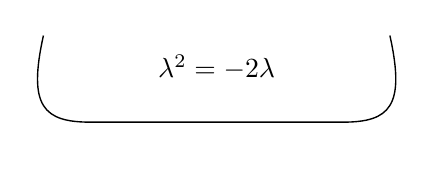
\begin{tikzpicture}[x=1mm,y=-1mm,line width=.5pt]
\path[use as bounding box](0,0)rectangle(48,15);
\node[inner sep=0]at(24,5){$\lambda^2=-2\lambda$};
\draw(2,1)..controls(0,10)and(2,12)..(8,12)--(40,12)..controls(46,12)and(48,10)..(46,1);
\end{tikzpicture}}
мульт. структура.
[Строка зачёркнута.]
\Unclear{GELFAND-P000059}{lower-cancellation}{Длинная густо зачёркнутая строка слева под формулами}
Есть
\SourceFigure{GELFAND-P000059}{inclusion-bars}{Над правой частью две горизонтальные черты разной длины и точка между ними.\par\smallskip\centering\color{black}\begin{tikzpicture}[x=1mm,y=-1mm,line width=.5pt]
\path[use as bounding box](0,0)rectangle(66,18);
\node[anchor=north west,inner sep=0]at(1,5){$\mathbf RP^{n-1}\subset O_n$};
\draw(49,3)--(54,3);\draw(58,2)--(65,2);\fill(56,2.7)circle(.3mm);
\end{tikzpicture}}
\par\noindent\begin{minipage}{\linewidth}
$S^n$ ставится на гиперпл. экватора $\longrightarrow$ в ортог. группу.
Кас. пучок --- отобр.
\Unclear{GELFAND-P000059}{sphere-map-insertion}{Над стрелкой тесно вставлено $\mathbf RP^{n-1}$ / $\mathbf RP^n$ с дополнительной наклонной стрелкой к $O_n$; часть знаков густая.\par\smallskip\centering\color{black}\begin{tikzpicture}[x=1mm,y=-1mm,line width=.5pt]
\path[use as bounding box](0,0)rectangle(65,24);
\node[inner sep=0]at(8,16){$S^{n-1}$};
\node[inner sep=0]at(53,16){$O_n$};
\node[inner sep=0]at(31,5){$\mathbf RP^{n-1}$};
\draw[->](20,16)--(43,16);\draw[->](42,8)--(48,13);
\end{tikzpicture}}
\end{minipage}\par
В симм. точках одинаков.
оно \uuline{2-листно}
(Склейка на экваторе)
вращение вокруг неё
\Unclear{GELFAND-P000059}{reflection-arrow}{От скобки об отражении стрелка вниз к $O(n)$; перед $O(n)$ чёрный переписанный штрих, чтение не установлено.\par\smallskip\centering\color{black}\begin{tikzpicture}[x=1mm,y=-1mm,line width=.5pt]
\path[use as bounding box](0,0)rectangle(73,27);
\node[anchor=north west,inner sep=0,text width=68mm]at(1,1){(отражение вокр. него)};
\draw[->](25,12)--(22,18);
\node[anchor=north west,inner sep=0]at(20,20){$O(n)$};
\end{tikzpicture}}
осей пр. пр-во.
\Unclear{GELFAND-P000059}{axis-name}{Альберт Солом. / Солн.}
Шварц.
\SourceFigure{GELFAND-P000059}{axis-diagram}{Наклонная прямая с точкой и подписью ось в $\mathbf R^n$.\par\smallskip\centering\color{black}\begin{tikzpicture}[x=1mm,y=-1mm,line width=.5pt]
\path[use as bounding box](0,0)rectangle(69,34);
\draw(5,32)--(24,1);\fill(15,16)circle(.7mm);
\node[anchor=north west,inner sep=0]at(27,2){ось в $\mathbf R^n$};
\end{tikzpicture}}
\par\noindent\begin{minipage}{\linewidth}
\begin{equation*}
\mathbf RP^{n-1}/\mathbf RP^{n-k-2}\longrightarrow O_n/O_{n-k-1}
\end{equation*}
\Unclear{GELFAND-P000059}{quotient-map}{В левом нижнем показателе $n-k-2$ / $n-n-2$; стрелка между факторами густо переписана.}
\end{minipage}\par
в действ. влож.

\Needspace{5\baselineskip}
\SourcePage{GELFAND-P000060}{unlabelled}
$1/\overline{\underline{\mathrm{III}}}$\par
\uwave{В.П. Паламодов.}
$\mathcal P$ --- кольцо мн. в $\mathbf C^n$,
$\mathcal J\subset\mathcal P$ --- идеал, примарный,
$P_1,\ldots,P_s$ --- образ.
\par\noindent\begin{minipage}{\linewidth}
$\mathcal H$ --- кольцо целых ф-й [знак зачёркнут] вып. области
\Unclear{GELFAND-P000060}{whole-functions-cancellation}{после «ф-й» густо зачёркнут короткий знак}
\end{minipage}\par
$\mathcal H/\mathcal J\mathcal H$ описывается так
\par\noindent\begin{minipage}{\linewidth}
\begin{equation*}
\mathcal H\{\mathcal J\}=\{f|_N\quad f(z)=d(z,\mathcal D)F_\zeta(z)\}
\end{equation*}
\Unclear{GELFAND-P000060}{local-f-index}{Нижний индекс $F$ похож на $\zeta$ / $s$.}
\end{minipage}\par
\par\noindent\begin{minipage}{\linewidth}
\begin{equation*}
\mathcal H/\mathcal J\mathcal H\cong\mathcal H\{\mathcal J\}\quad^{\text{лок. часть}}
\end{equation*}
\EvidenceBlock{GELFAND-P000060}{local-part}{Помета «лок. часть» стоит справа вверху от второй формулы.}{Положение пометы.}
\end{minipage}\par
каждан гов., что $\underset{\longrightarrow}{\text{это}}$ \underline{получ.} алгебраически.

$\bullet$ \underline{Гельфанд.}
\uwave{Пример Нельсона.}
2 самосопр. оператора $A$ и $B$.
что меняет самосопр. опер.? (не симм. замкн.)
[На правом поле:]
\par\noindent\begin{minipage}{\linewidth}
\begin{equation*}
i\frac d{dx},\qquad y(a)=y(b)
\end{equation*}
\Unclear{GELFAND-P000060}{boundary-margin}{Ниже написано «или ещё $=0$»; перед знаком равенства аргумент не указан.}
\end{minipage}\par
По существу самосопр. $A$ (симм.), если
нет вект., ортог. ко всем вект. вида
\par\noindent\begin{minipage}{\linewidth}
\begin{equation*}
\overline z=Ax-ix,\qquad z=Ax+ix
\end{equation*}
\Unclear{GELFAND-P000060}{range-z-marks}{У первого $z$ длинная верхняя черта. У второго верхний штрих может быть частью буквы или отдельной пометой.}
\end{minipage}\par
\par\noindent\begin{minipage}{\linewidth}
(Тогда [запись зачёркнута] то же $\forall$ компл. $\lambda$)
\Unclear{GELFAND-P000060}{criterion-cancellation}{короткая густая отмена}
\end{minipage}\par
иначе $Ax-ix$ всюду плотны
$A-iE$ им. обр. (в общем?: если замкнуты)
\par\noindent\begin{minipage}{\linewidth}
\begin{equation*}
\left(i\frac d{dx}\quad\text{[на / не] даже аналит.}\quad
\begin{array}{ll}
f(a)=f(b)&\text{\uwave{по сущ. самосопр.}}\\
f(a)=f(b)=0&\text{только симм.}
\end{array}\right)
\end{equation*}
\Unclear{GELFAND-P000060}{differential-qualifier}{Перед условиями написано «[на / не] даже аналит.»; последняя буква первого слова слита.}
\end{minipage}\par
$A$ и $B$ по существу самосопр.,
$\alpha A+\beta B$ по сущ. самосопр.,
$\alpha,\beta$ --- вещ.
\begin{equation*}
\forall f\in\text{обл. опред.}\qquad ABf=BAf.
\end{equation*}
\Unclear{GELFAND-P000060}{domain-cancellation}{Над областью определения густо переписана короткая запись; под ней изогнутая черта.\par\smallskip\centering\color{black}\begin{tikzpicture}[x=1mm,y=-1mm,line width=.5pt]
\path[use as bounding box](0,0)rectangle(32,9);
\draw(1,1)..controls(2,9)and(7,8)..(11,6)..controls(15,10)and(20,4)..(30,2);
\end{tikzpicture}}
Тем не менее $A$ и $B$ не перестановочны.
\SourceFigure{GELFAND-P000060}{example-emphasis}{Слева зачёркнуто и дважды подчёркнуто «Пример.»; справа от него двойная вертикальная черта.\par\smallskip\centering\color{black}\begin{tikzpicture}[x=1mm,y=-1mm,line width=.5pt]
\path[use as bounding box](0,0)rectangle(48,25);
\node[anchor=north west,inner sep=0]at(1,2){\uuline{\sout{Пример.}}};
\draw(39,2)--(39,24);\draw(41,2)--(41,24);
\end{tikzpicture}}
$A$ и $B$ перест., если разумн. ф-и от них перестан.
\par\noindent\begin{minipage}{\linewidth}
\begin{equation*}
\underset{\text{опер. ограничен}}{(A-\lambda E)^{-1}}
\end{equation*}
\Unclear{GELFAND-P000060}{resolvent-understroke}{Под $\lambda E$ нижние штрихи; отдельное подчёркивание или части букв, не установлено.}
\end{minipage}\par
\par\noindent\begin{minipage}{\linewidth}
Перест. [Зачёркнуто: \textcolor{orange!65!black}{не...}] и с $B$ означает, что и эти опер. перестан.
\Unclear{GELFAND-P000060}{resolvent-cancellation}{Начало зачёркнутой записи похоже на «не»; дальнейшие буквы скрыты.}
\end{minipage}\par
\begin{equation*}
e^{iA}\quad\text{--- унит.}\qquad e^{iB}\quad\text{не перестановочны}
\end{equation*}
\par\noindent\begin{minipage}{\linewidth}
[Запись зачёркнута; рядом $(\forall\text{ огр. опер.})$.]
\Unclear{GELFAND-P000060}{final-cancellation}{Короткая густо зачёркнутая запись}
\end{minipage}\par

\Needspace{5\baselineskip}
\par\noindent\begin{minipage}{\linewidth}
\SourcePage{GELFAND-P000061}{42}
\uuline{Пример Нелсона.}
\SourceFigure{GELFAND-P000061}{nelson-grid}{Квадратная сетка, жирные точки и центральная штриховка; подписи $0,1,2,3$ снизу, $1,2,3$ слева и $2$ справа. Между $1$ и $2$ слева знак похож на $3$, нижний штрих густой; центральные наложенные штрихи и точная склейка не установлены.\par\smallskip\centering\color{black}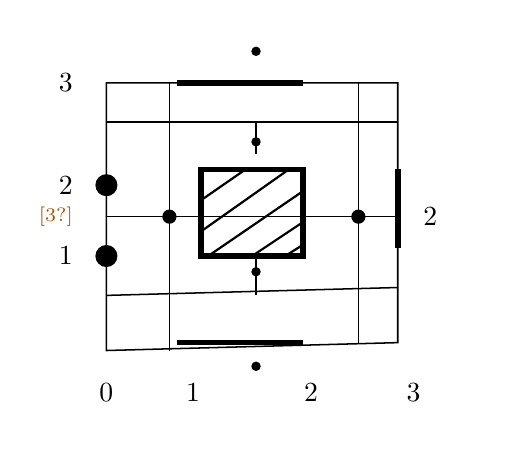
\begin{tikzpicture}[x=1mm,y=-1mm,line width=.55pt]
\path[use as bounding box](0,0)rectangle(58,53);
\draw(10,7)--(47,7)--(47,40)--(10,41)--cycle;
\draw(18,7)--(18,41);\draw(42,7)--(42,40);
\draw(10,12)--(47,12);\draw(10,24)--(47,24);\draw(10,34)--(47,33);
\draw(29,12)--(29,16);\draw(29,29)--(29,34);
\draw[line width=2pt](19,7)--(35,7);\draw[line width=2pt](19,40)--(35,40);
\draw[line width=2pt](47,18)--(47,28);
\fill(10,20)circle(1.4);\fill(10,29)circle(1.4);
\fill(18,24)circle(.9);\fill(42,24)circle(.9);
\fill(29,14.5)circle(.6);\fill(29,31)circle(.6);
\draw[line width=2.1pt](22,18)--(35,18)--(35,29)--(22,29)--cycle;
\begin{scope}\clip(22,18)rectangle(35,29);
\draw[line width=.8pt](19,24)--(32,15);\draw[line width=.8pt](19,28)--(36,16);
\draw[line width=.8pt](20,31)--(39,18);\draw[line width=.8pt](24,32)--(39,22);
\draw[line width=.8pt](28,32)--(39,25);\end{scope}
\node[anchor=east]at(7,7){$3$};\node[anchor=east]at(7,20){$2$};
\node[anchor=east]at(7,29){$1$};\node[anchor=east]at(7,24){\scriptsize\textcolor{orange!65!black}{[$3$?]}};
\node[anchor=north]at(10,44){$0$};\node[anchor=north]at(21,44){$1$};
\node[anchor=north]at(36,44){$2$};\node[anchor=north]at(49,44){$3$};
\node[anchor=west]at(49,24){$2$};\fill(29,3)circle(.6);\fill(29,43)circle(.6);
\end{tikzpicture}}
\end{minipage}\par
Из обл. между квадр. выбр. жирные точки
Отрезки склеиваются
кажд. точка склеив. с точкой гран. ближ. по гориз. или верт.
Углы склеив. между собой. Получ. поверхн. рода
\textcolor{orange!65!black}{$\underline{4}$}
с одной выбр. точкой
\Unclear{GELFAND-P000061}{genus}{В цифре видны угловатый верх и широкая нижняя черта. Чтение $4$ предпочтительно, возможно $1$.}
\par\noindent\begin{minipage}{\linewidth}
\begin{equation*}
X=\frac{d}{dx},\qquad y=\frac{d}{dy}
\end{equation*}
\Unclear{GELFAND-P000061}{generator-symbol}{У второго знака слева от равенства нижняя петля, как у $y$; далее написано $iY$.}
\end{minipage}\par
$iX$, $iY$ --- формально самосопр.
Они коммутируют
Но соотв. опер. не коммут.
Выбр. меры $0$ замкн. траект. попад. в вершины.
$e^X$ и $e^Y$ --- унит. опер., к-рые не перестановочны.
\begin{equation*}
e^{\frac{d}{dx}}f(x)=f(x+1)
\end{equation*}
(ф-ла Тейлора)
Док. сначала для аналит. ф-й, потом для всего гильб.
пр-ва пред. перех. (опер. унитарный)
И надо её двигать.
\SourceFigure{GELFAND-P000061}{shift-square}{Квадрат с отверстием; штриховка слева от отверстия и в нижнем левом участке, два коротких штриха справа от него. Наклонная черта идёт от нижнего левого участка вниз к подписи. Границы наложенных штрихов не установлены.\par\smallskip\centering\color{black}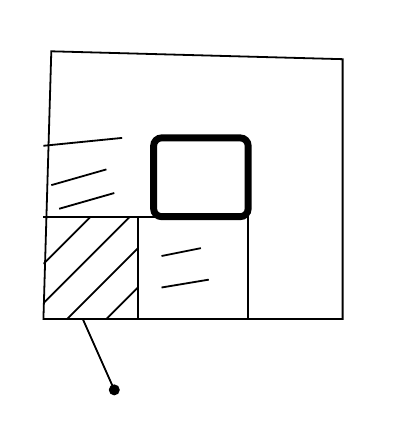
\begin{tikzpicture}[x=1mm,y=-1mm,line width=.65pt]
\path[use as bounding box](-2,-2)rectangle(44,47);
\draw(1,1)--(38,2)--(38,35)--(0,35)--cycle;
\draw(0,22)--(26,22)--(26,35);\draw(12,22)--(12,35);
\draw[line width=2.5pt,rounded corners=1mm](14,12)rectangle(26,22);
\draw(0,13)--(10,12);\draw(1,18)--(8,16);\draw(2,21)--(9,19);
\begin{scope}\clip(0,22)rectangle(12,35);
\draw(0,28)--(6,22);\draw(0,33)--(11,22);\draw(3,35)--(12,26);\draw(8,35)--(12,31);
\end{scope}
\draw(15,27)--(20,26);\draw(15,31)--(21,30);
\draw(5,35)--(9,44);\fill(9,44)circle(.7);
\end{tikzpicture}}
$e^Y$ --- обл. на $1$ вверх, $e^X$ прокрутится
\begin{equation*}e^X\end{equation*}
ф-я с \textcolor{orange!65!black}{компт.} здесь.
\Unclear{GELFAND-P000061}{support-word}{компт. / комп.}
Исключ. конечн. число траект.
$e^{tX}$ --- сдвиг по траект. опер. $X$
локально всюду перестановочны
\par\noindent\begin{minipage}{\linewidth}
что будет с [Вставлено сверху: с] опер. Лапласа?
\EvidenceBlock{GELFAND-P000061}{laplace-overwrite}{«с» написано над отметкой вставки.}{Вставка в рукописи.}
\end{minipage}\par
индекс дефекта
\begin{gather*}
\Delta f=if\\
\underline{\Delta=X^2+Y^2}
\end{gather*}
(это след. из теор. Нелсона)
Он не явл. самосопр. (имеет решение $C^\infty$, гр. усл., а в точке только $\int$ квадрат.)
Сами опер. сдвига опр. на $L^2$, а не на периодич. ф-ях.
\underline{3 опр}
$e^{itA}$:
\par\noindent\begin{minipage}{\linewidth}
\begin{align*}
1^\circ&=\int_{-\infty}^{+\infty}\frac{e^{it\lambda}}{iA-\lambda}\,d\lambda\\
2^\circ&=\int_{-\infty}^{+\infty}e^{it\lambda}\,dE_\lambda\\
3^\circ&:\quad \frac{df}{dt}=iAf
\end{align*}
\Unclear{GELFAND-P000061}{resolvent}{В первой записи знаменатель $iA-\lambda$; отдельного множителя перед интегралом не видно.}
\Unclear{GELFAND-P000061}{evolution-prefix}{Перед дробью в третьей строке короткий тёмный штрих; точное чтение не установлено.}
\end{minipage}\par
$\underset{\text{реш.}}{U}_{t,0}f_0=f$ --- унит. опер.

\Needspace{5\baselineskip}
\SourcePage{GELFAND-P000062}{unlabelled}
\uwave{Синай.} \uwave{Полож. в дин. системах.}
У эргод. дин. сист.
[Зачёркнуто: короткая густо зачёркнутая запись; вставлено сверху: с дискр. сп.]
спектр всегда простой
\Unclear{GELFAND-P000062}{cancelled-spectrum}{короткая густо зачёркнутая запись}
$M$, $\mu$, $\{S_t\}$ --- однопар. гр. в $M$
В $\mathcal L^2_\mu$
однопар. гр. унит. опер.
\par\noindent\begin{minipage}{\linewidth}
\begin{equation*}
\underset{\tikz[baseline=-.5ex]{\draw[->] (0,1.7mm) .. controls (2mm,0) and (7mm,0) .. (9mm,1.7mm);}}{U_t}f(x)=f(S_t x)
\end{equation*}
\EvidenceBlock{GELFAND-P000062}{operator-curve}{Под $U_t$ дуга с остриём справа; «простое» относится к следующей строке.}{Знак рукописи.}
\end{minipage}\par
В эргод. случае каждое соб. знач. простое
\uwave{Лебеговский спектр:}
$\forall f$
\begin{equation*}
(U_t f,f)=\int e^{it\lambda}p(\lambda)\,d\lambda
\end{equation*}
($p(\lambda)$ --- суммир.)
(Вообще всегда $\int e^{it\lambda}\,d\mu$, здесь $\mu$ абс. непр.)
\uwave{Счётнокр. леб. сп.}:
$\exists$ ортог. $f_1,f_2,\ldots$
\begin{equation*}
(U_t f_i,f_j)=0\qquad(i\neq j)
\end{equation*}
и всё порожд.
Во всех изв. прим. спектр счётно-кр.
\underline{Прим.} \uwave{Пр. тора.}
\begin{equation*}
\begin{pmatrix}a&b\\c&d\end{pmatrix},
\qquad \det=1,\quad\text{целочисл.}
\end{equation*}
\begin{gather*}
x\longrightarrow ax+by\\
y\longrightarrow cx+dy
\end{gather*}
Надо найти авток. Разлож. в ряд Фурье и действ.
\begin{gather*}
f(x,y)\longrightarrow f(ax+by,cx+dy)\\
e^{2\pi i(mx+ny)}
\longrightarrow e^{2\pi i((am+cn)x+(bm+dn)y)}
\end{gather*}
На целочисл. реш. действует матрица.
Надо взять траектории
\begin{equation*}
(m,n)\longrightarrow S(m,n)=(m',n')
\end{equation*}
Траект. --- гипербола.
\SourceFigure{GELFAND-P000062}{hyperbola}{Сверху пересекаются два штриха без явных стрелок. Ниже наклонная линия и два изогнутых штриха; утолщение в пересечении. Концы наклонной линии справа вверху и длинного изогнутого штриха внизу похожи на стрелки; принадлежность наложенных штрихов не установлена.\par\smallskip\centering\color{black}\begin{tikzpicture}[x=1mm,y=-1mm,line width=.6pt]
\path[use as bounding box](0,0)rectangle(43,23);
\draw(3,14)..controls(17,14)and(29,14)..(40,12);
\draw(16,2)--(18,21);
\end{tikzpicture}
\par\smallskip
\begin{tikzpicture}[x=1mm,y=-1mm,line width=.65pt]
\path[use as bounding box](0,0)rectangle(48,58);
\draw[->](3,52)--(44,15);
\draw[->](16,5)..controls(20,21)and(22,31)..(27,55);
\draw(21,2)..controls(22,15)and(25,33)..(35,24)..controls(37,22)and(38,20)..(39,18);
\draw[line width=1.7pt](22,29)--(24,34);
\end{tikzpicture}}
Вещ. соб. знач. --- сж. по одной оси
и растяж. по др. ($\det=1$)
\par\noindent\begin{minipage}{\linewidth}
\begin{equation*}
S^k\left(\frac mn\right)\longrightarrow\lambda
\end{equation*}
($\lambda$ --- соб. знач.)
\Unclear{GELFAND-P000062}{frequency-limit}{Между $m$ и $n$ горизонтальная черта. Справа стрелка к $\lambda$; дополнительного множителя не видно.}
\end{minipage}\par
Волны стан. всё более густыми и напр.
Волны $\Longrightarrow$ к соб. напр.
Пр-во разлож. на пр-во ф-й с частотами на
гиперболах. На $1$-й гиперболе.
Послед. ортог. вект., кажд. перех. в следующий

\Needspace{5\baselineskip}
\SourcePage{GELFAND-P000063}{43}
\SourceFigure{GELFAND-P000063}{shift-points}{Сверху ряд из девяти отдельных точек.\par\smallskip\centering\color{black}\begin{tikzpicture}[x=1mm,y=1mm]
\path[use as bounding box](0,-2)rectangle(71,3);
\fill(2,0)circle(.45);\fill(10,.4)circle(.6);\fill(18.7,.3)circle(.55);
\fill(27.4,.1)circle(.5);\fill(34.7,.5)circle(.35);\fill(42.1,.6)circle(.35);
\fill(50.1,.3)circle(.4);\fill(55.5,.2)circle(.3);\fill(65.2,.5)circle(.35);
\end{tikzpicture}}
(сдвиг на $1$ в целочисл. т.)
непр. лебеговский спектр. Со сх. Бернулли --- характ. группы.
\uwave{Теорема.} Мера $d\sigma(\lambda)$
\SourceFigure{GELFAND-P000063}{spectral-axes}{Два пересекающихся штриха; стрелки вправо и вверх. Подписей нет.\par\smallskip\centering\color{black}\begin{tikzpicture}[x=1mm,y=1mm,line width=.7pt]
\path[use as bounding box](-20,-15)rectangle(23,15);
\draw[->](-18,0)--(21,0);\draw[->](0,-13)--(0,13);
\end{tikzpicture}}
$\sigma\times\sigma$
\par\noindent\begin{minipage}{\linewidth}
\begin{gather*}
\alpha=\lambda_1+\lambda_2\\
\beta=\lambda_1-\lambda_2\\
\text{мера}\quad d\sigma(\lambda_1)\times d\sigma(\lambda_2)=\underbrace{d\sigma^2(\alpha)}_{\text{свёртка}}
\end{gather*}
\Unclear{GELFAND-P000063}{spectral-product}{После произведения мер написано $d\sigma^2(\alpha)$, ниже «свёртка»; отдельного множителя по $\beta$ не видно.}
\end{minipage}\par
\textcolor{orange!65!black}{$8/\overline{\underline{\mathrm{III}}}$ \underline{Я. Синай.}}
\Unclear{GELFAND-P000063}{date-sinai}{Перед $/\overline{\underline{\mathrm{III}}}$ густо переписанный знак: $8$ / $4$ / $1$; ниже \underline{Я. Синай} / \underline{2. Синай}.}
\SourceFigure{GELFAND-P000063}{intermediate-marks}{Короткая горизонтальная черта, отдельная точка, более длинная почти горизонтальная черта.\par\smallskip\centering\color{black}\begin{tikzpicture}[x=1mm,y=1mm,line width=.6pt]
\path[use as bounding box](0,-2)rectangle(40,3);
\draw(1,0)--(10,0);\fill(17,.1)circle(.4);\draw(25,.2)--(39,.5);
\end{tikzpicture}}
$M,\mu,\{S_t\}$.
Соб. ф-я
\begin{equation*}
U_t f_\lambda=e^{i\lambda t}f_\lambda
\end{equation*}
пост. по \uuline{mod} (у эргод. системы)
$15/\overline{\underline{\mathrm{III}}}$ \underline{Тодоров} $SU$
$22/\overline{\underline{\mathrm{III}}}$-$65$ \uwave{Через год в Москве будет матем. конгресс.}
(март --- апрель)
[что такое «простой корень»? связь с матрицами]
\underline{Гелф.} \underline{Зад.}
1. Делать алг. геом. на некомм. кольцах!!
2. Алг. теор. дифф. ур-й.
\underline{Повзнер.} Малый параметр.
\underline{Березин.} О ф-ях многих переменных.
Надо изуч. не все ф-и, а специф. --- встр. в теор. предст. и
в стат. физике.
\underline{Повзнер} «пожелание» к Березину.
\uuline{Кириллов.}
Обычн. дин. сист. --- время $R$ или $Z$. Можно
произв. группа сохр. меру. Классифик., инвар.?
[Перед «Спектр» зачёркнуто: короткая запись под густыми штрихами.]
\Unclear{GELFAND-P000063}{cancelled-spectrum}{короткая запись под густыми штрихами}
Спектр --- мн-во неприв. предст., на к-рые
разлож. пр-во ф-й на $M$
\begin{equation*}
\begin{array}{ll}
M&G\\
\underset{\text{ф-и}}{H}&\underset{\text{унит. опер.}}{U_g:f(x)\longrightarrow f(g^{-1}x)}
\end{array}
\end{equation*}
$H$ разлож. на неприв. компон., к-рые наз. спектром.
$G$ комм. --- прдпр. одномерны.
$G$ действ. эргодич. (нет инв. ф-й, кроме const)
Для комп. гр. Все \underline{транзит.} и св. к описанию
подгрупп.
\underline{Прим.} 1) \uwave{Гордин и Уайтхед.}
\par\noindent\begin{minipage}{\linewidth}
\begin{equation*}
G=\prod Z_2
\end{equation*}
\EvidenceBlock{GELFAND-P000063}{group-product}{Записан знак произведения. В следующей строке указано конечное число ненулевых членов.}{Запись в рукописи.}
\end{minipage}\par
\uwave{Некомп. группа}
Послед. $0$ и $1$, конечн. число не $0$.
$\sum$ обычн.
У неё реш. зад. опис. предст. вирт. подгруппы

\Needspace{5\baselineskip}
\SourcePage{GELFAND-P000064}{unlabelled}
2) Двоично-рац. числа на окр.
\begin{equation*}
\underline{e^{i\frac{\pi k}{2^n}}}
\end{equation*}
\Unclear{GELFAND-P000064}{dyadic-exponent}{Перед $k$ виден знак, похожий на $\pi$; отдельное $2$ не различимо. Чтения $\pi k$ / $2\pi k$.}
Счётная.
Двойств. гр. --- 2-адич. числа.
\par\noindent\begin{minipage}{\linewidth}
На ней уже \textcolor{orange!65!black}{некл.} факты.
\Unclear{GELFAND-P000064}{nonclassical}{Перед «факты» сокращение похоже на «некл.»; последние штрихи слиты.}
\end{minipage}\par
Точ. спектр и непр. сп.
Возм., что [зачёркнуто:
ф / неразборчиво]
произв. ф-й, разлож. по участкам.
\Unclear{GELFAND-P000064}{cancelled-function}{ф / неразборчиво}
\SourceFigure{GELFAND-P000064}{sawtooth}{Два коротких пилообразных участка над горизонтальными подчёркиваниями; крайние штрихи и некоторые изломы неуверенны.\par\smallskip\centering\color{black}\begin{tikzpicture}[x=.96mm,y=.96mm,line width=.7pt]
\path[use as bounding box](0,-5)rectangle(83,16);
\draw(3,4)--(3,13);\draw(3,8)..controls(6,12)and(8,13)..(9,9)..controls(10,6)and(13,7)..(16,11)..controls(16,6)and(19,6)..(23,10)..controls(23,6)and(29,7)..(34,9);
\draw(34,5)--(34,13);\draw(3,-2)..controls(10,-1)and(20,-2)..(29,-1);
\draw(52,6)--(52,13);\draw(52,10)..controls(54,15)and(55,12)..(55,8)..controls(58,8)and(59,9)..(60,11)..controls(60,5)and(63,6)..(65,10)..controls(67,4)and(72,6)..(77,8);
\draw(77,4)--(78,14);\draw(50,-2)..controls(59,-2)and(69,-4)..(83,-2);
\end{tikzpicture}}
Непр. сп. даёт ф-ю разлож.
по дискр. мн-ву.
\uwave{Оследец}: было и для обычн. системы.
\uwave{2-мерн. время.}
\par\noindent\begin{minipage}{\linewidth}
\begin{equation*}
\begin{pmatrix}a&b\\0&1\end{pmatrix}
\end{equation*}
\SourceFigure{GELFAND-P000064}{affine-matrix-underline}{Под матрицей длинное двойное подчёркивание с косыми штрихами.\par\smallskip\centering\color{black}\begin{tikzpicture}[x=1mm,y=1mm,line width=.7pt]
\path[use as bounding box](0,-2)rectangle(47,5);
\draw(1,2)--(45,4)--(46,2)--(0,0)--(3,3)--(44,3);
\draw(3,0)--(7,3)--(9,0)--(13,3)--(15,1)--(19,3)--(21,1)--(25,3)--(27,1)--(31,3)--(33,1)--(37,3)--(39,2);
\end{tikzpicture}}
\end{minipage}\par
Потоки Синая (оснащённые).
Непр. предст. мало:
одном. $|a|^{i\lambda}(\operatorname{sign}a)^\varepsilon$!
И одно беск.-мерное.
\uwave{Связь с группой Лоренца.}
\SourceFigure{GELFAND-P000064}{lorentz-emphasis}{Волнистое подчёркивание; под «с» короткий нисходящий штрих с изломом.\par\smallskip\centering\color{black}\begin{tikzpicture}[x=1mm,y=1mm,line width=.7pt]
\path[use as bounding box](0,-5)rectangle(76,4);
\draw(0,0)..controls(3,3)and(5,3)..(7,1)..controls(9,-1)and(11,-1)..(14,1)..controls(17,3)and(19,2)..(21,0)..controls(24,-1)and(27,2)..(31,2)..controls(35,2)and(38,-1)..(42,0)..controls(47,3)and(52,3)..(56,1)..controls(61,-1)and(66,2)..(70,1)..controls(73,0)and(74,1)..(76,2);
\draw(16,3)--(17,-3)--(15,-1);\draw(17,-3)--(17,0);
\end{tikzpicture}}
\begin{equation*}
\begin{pmatrix}a&b\\c&d\end{pmatrix}
\end{equation*}
Действ. на пр-ве Лобач. (верхн. полуплоскость).
Про факт. по [зачёркнуто:
неразборчиво]
дискр. подгр. Будет комп. отриц. крив.
\Unclear{GELFAND-P000064}{cancelled-discrete}{неразборчиво}
Кас. пучок --- 3-х мерн. комп. мн., на к-ром действует
эргодич. гр. Лоренца.
Дискр. спектр из-за компактности.
\uwave{Гомологии дин. систем.}
Оператор
\begin{equation*}
U_g=\alpha(x,g)f(xg).
\end{equation*}
Гомоморфизм тогда.
$\alpha(x,g)$ --- коцикл. $|\alpha|=1$.
\begin{equation*}
\alpha\in Z^1(G,\underset{\substack{\vert\\\text{гр. функций}}}{F}).
\end{equation*}
\par\noindent\begin{minipage}{\linewidth}
$\alpha$ эквив., если сущ. перев. преобр.
\EvidenceBlock{GELFAND-P000064}{equivalence}{Видно сокращение «перев.» перед «преобр.».}{Запись в рукописи.}
\end{minipage}\par
Это быв., если
\begin{equation*}
\frac{\alpha}{\alpha_1}\in B^1(G,F)
\end{equation*}
Общ. вид границы
\begin{equation*}
\alpha_0(x,g)=\frac{\beta(xg)}{\beta(x)}
\end{equation*}
--- гомолог. нулю.
$Z^1/B^1$ --- гомологии.
Выч. лишь если гр. транзитивна (тогда
это мн-во предст. стаб. подгруппы).
\par\noindent\begin{minipage}{\linewidth}
Гом. 0 не все const, а $e^{2\pi i\lambda}$.
\EvidenceBlock{GELFAND-P000064}{zero-hom}{После $i$ сразу стоит $\lambda$.}{Запись в рукописи.}
\end{minipage}\par
\SourceFigure{GELFAND-P000064}{spectrum-caption-stroke}{Справа подпись с длинным изогнутым подчёркиванием.\par\smallskip\centering\color{black}\begin{tikzpicture}[x=1mm,y=1mm,line width=.7pt]
\path[use as bounding box](0,-3)rectangle(53,8);
\node[anchor=west,inner sep=0pt]at(0,5){$\lambda$ из спектра.};
\draw(2,1)..controls(6,-2)and(13,-1)..(25,-1)..controls(36,-1)and(44,0)..(53,-2);
\end{tikzpicture}}
\par\noindent\begin{minipage}{\linewidth}
Есть подозр., что
гр. гом. опред. дин. систему.
\EvidenceBlock{GELFAND-P000064}{conjecture}{Заключение начинается словами «Есть подозр., что».}{Запись в рукописи.}
\end{minipage}\par

\Needspace{5\baselineskip}
